\documentclass[a4paper,11pt,notitlepage]{report}

\usepackage{graphicx}
\usepackage[utf8]{inputenc}
\usepackage[T1]{fontenc}
\usepackage[ngerman]{babel}
\usepackage{bibgerm}
\usepackage{amsmath,amssymb,amsthm}
\usepackage{color}
\usepackage{enumerate}
\usepackage{tabularx}
\usepackage{subfig}
\usepackage{fancyhdr}
\usepackage{upgreek}
\usepackage[pdftex,pdfpagelabels,colorlinks,backref,pagebackref]{hyperref}
\usepackage{tikz} % SELBST HINZUGEFÜGT
\usepackage{graphicx}
\usepackage{framed}
\usepackage{lmodern}
% == Set the heading style ===================================================
\setlength{\headheight}{14pt}
\pagestyle{fancyplain}
\renewcommand{\chaptermark}[1]{\markboth{#1}{}}
\renewcommand{\sectionmark}[1]{\markright{\thesection\ #1}}
\lhead[\fancyplain{}{\thepage}]{\fancyplain{}{\rightmark}}
\rhead[\fancyplain{}{\leftmark}]{\fancyplain{}{\thepage}}
\cfoot{}
\renewcommand{\headrulewidth}{0.4pt}
% ============================================================================

% == Set correct values for fitting floats ===================================
\tolerance=2000
\emergencystretch=10pt

\setcounter{topnumber}{3}
\setcounter{totalnumber}{5}
\setcounter{bottomnumber}{2}

% To make those darn floats fit where they should
\setcounter{totalnumber}{9}
\setcounter{topnumber}{9}
\setcounter{bottomnumber}{9}
\renewcommand{\textfraction}{0.00}
\renewcommand{\topfraction}{1.0}
\renewcommand{\bottomfraction}{1.0}
% ============================================================================

% == German definitions for theorems etc. ==================================== 
\newtheorem{definition}{Definition}[chapter]
\newtheorem{theorem}{Satz}[chapter]
\newtheorem{lemma}{Lemma}[chapter]
\newtheorem{proposition}{Proposition}[chapter]
\newtheorem{corollary}{Korollar}[chapter]
\newtheorem{observation}{Beobachtung}[chapter]
\newtheorem{fact}{Fakt}[chapter]
\newtheorem{remark}{Bemerkung}[chapter]
\newtheorem{example}{Beispiel}[chapter]
% ============================================================================

% == Abkürzungen für die reellen, natürlichen, ganzen,... Zahlen =============
\newcommand{\R}{{\ensuremath{\mathbb{R}}}}
\newcommand{\N}{{\ensuremath{\mathbb{N}}}}
\newcommand{\Z}{{\ensuremath{\mathbb{Z}}}}
\newcommand{\C}{{\ensuremath{\mathbb{C}}}}
\newcommand{\Q}{{\ensuremath{\mathbb{Q}}}}
\newcommand{\F}{{\ensuremath{\mathbb{F}}}}
\newcommand{\Prim}{{\ensuremath{\mathbb{P}}}}
% ============================================================================

% == Makros für Autorenname und -adresse =====================================
\newcommand{\myaddress}[6]{%
  \parbox{\textwidth}{\textbf{\large #1}\\
    #2\\ #3\\ #4\\ 
    \ifthenelse{\equal{#5}{}}{}{Email: \href{mailto:#5}{\texttt{#5}}\\}
    \ifthenelse{\equal{#6}{}}{}{WWW: \href{#6}{\path|#6|}\\}
  } 
}

\newcommand{\myauthor}[1]{%
  \addtocontents{toc}{\protect\hspace{3.35ex}%
  \textsl{#1}\par}\vspace{-4ex}\quad\hfill\textsl{\Large #1}\vspace{8ex}}

\newcommand{\myname}[1]{\Large #1}

%%%%%%%%%%%%%%%%%%%%%%%%%%%%%%%%%%%%%%%%%%%%%%%%%%
% Tragen Sie in der folg. Zeile Ihren Namen ein: %
%%%%%%%%%%%%%%%%%%%%%%%%%%%%%%%%%%%%%%%%%%%%%%%%%%

\newcommand{\OO}{{\ensuremath{\mathcal{O}}}}

\renewcommand{\thechapter}{\Roman{chapter}}
\renewcommand{\thesection}{\arabic{section}}


\newenvironment{Kasten}[1]
{
\hspace{0.05\linewidth}
\begin{center}
\begin{minipage}{0.9\linewidth}
\setlength{\fboxsep}{10pt}
%\setlength{\fboxsep}{18pt}
%\definecolor{shadecolor}{gray}{0.9}
\definecolor{shadecolor}{gray}{1}
\definecolor{framecolor}{gray}{0}
\def\FrameCommand{\fcolorbox{framecolor}{shadecolor}}
\MakeFramed {\FrameRestore}
\subsection{#1}
\begin{itshape}
}
{
\end{itshape}
\endMakeFramed
\end{minipage}
\end{center}
%\vspace{1em}
}

\begin{document}
\shorthandoff{"}
\setcounter{chapter}{0}

\begin{titlepage}
	\begin{center}	
		\LARGE \textbf{{Einführung in die Geometrie und Topologie - Mitschrieb -} \\[5ex] 
    		{\Large Vorlesung im Wintersemester 2011/2012\\[5ex]}}
	\end{center}
	\begin{center}
		\Large Sarah Lutteropp, Simon Bischof
	\end{center}
	\begin{center}
		\today
	\end{center}
	\vspace{2cm}
	\begin{center}
		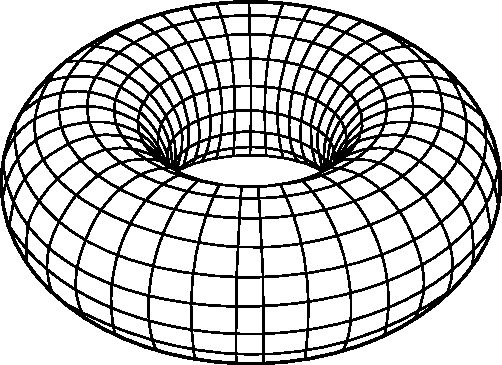
\includegraphics[width=0.8\textwidth]{torus2.pdf}
	\end{center}
\end{titlepage}
%\maketitle
\setcounter{tocdepth}{1}
\tableofcontents

\section*{Zusammenfassung}
Dies ist ein Mitschrieb der Vorlesung “Einführung in die Geometrie und Topologie” vom Wintersemester 2011/2012 am Karlsruher Institut für Technologie, die von Herrn Prof. Dr. Wilderich Tuschmann gehalten wird.

\chapter{Homotopie und Fundamentalgruppe}
\setcounter{section}{-1}
\section{Vorwort}
\begin{Kasten}{Topologischer Raum}
Ein \underline{topologischer Raum} $X$ ist gegeben durch eine Menge $X$ und ein System $\OO$ von Teilmengen von $X$, den so genannten \underline{offenen Mengen} von $X$, welches unter beliebigen Vereinigungen und endlichen Durchschnitten abgeschlossen ist und $X$ und die leere Menge $\emptyset$ als Elemente enthält.
\newline
$X$ Menge, $\OO \subset \mathcal{P}(X) \colon$
\begin{enumerate}[(1)]
	\item $O_1, O_2 \in \OO \Rightarrow O_1 \cap O_2 \in \OO$
	\item $O_\alpha \in \OO, \alpha \in A, A \text{ Indexmenge} \Rightarrow \bigcup\limits_{\alpha \in A}{O_\alpha} \in \OO$
	\item $X, \emptyset \in \OO$
\end{enumerate}
\end{Kasten}

\begin{example}
\OO = $\{X, \emptyset\} \Rightarrow (X,\OO)$ ist topologischer Raum!
\end{example}

\begin{example}
$$X \text{ Menge, }\OO = \left\{\{x\} \mid x\in X\right\} + \text{Axiome, die zu erfüllen sind} \leadsto \tilde{\OO} = \mathcal{P}(X)$$
$\Rightarrow (X,\tilde{\OO})$ ist topologischer Raum.
$\OO$ ist "Basis" der Topologie $\tilde{\OO}$.
\end{example}

\begin{Kasten}{Metrischer Raum}
Ein \underline{metrischer Raum} $X$ ist eine Menge $X$ mit einer Abbildung $d \colon X \times X \rightarrow \R$, der \underline{"Metrik"} auf $X$, die folgende Eigenschaften erfüllt:
$\forall x,y,z \in X$
\begin{enumerate}[(1)]
	\item $d(x,y) = d(y,x)$ \underline{"Symmetrie"}
	\item $d(x,y) = 0 \Leftrightarrow x = y, d(x,y) \geq 0$ \underline{"Definitheit"}
	\item $d(x,z) \leq d(x,y) + d(y,z)$ \underline{"Dreiecksungleichung"}
\end{enumerate}
\end{Kasten}

%\begin{Kasten}[stetig]
\begin{Kasten}{Stetigkeit}
Eine Abbildung $F \colon X \rightarrow Y$ zwischen topologischen Räumen $X$ und $Y$ heißt \underline{stetig}, falls die F-Urbilder offener Mengen in $Y$ offene Teilmengen von $X$ sind.
%\end{Kasten}
\end{Kasten}

\begin{figure}[h]
\centering
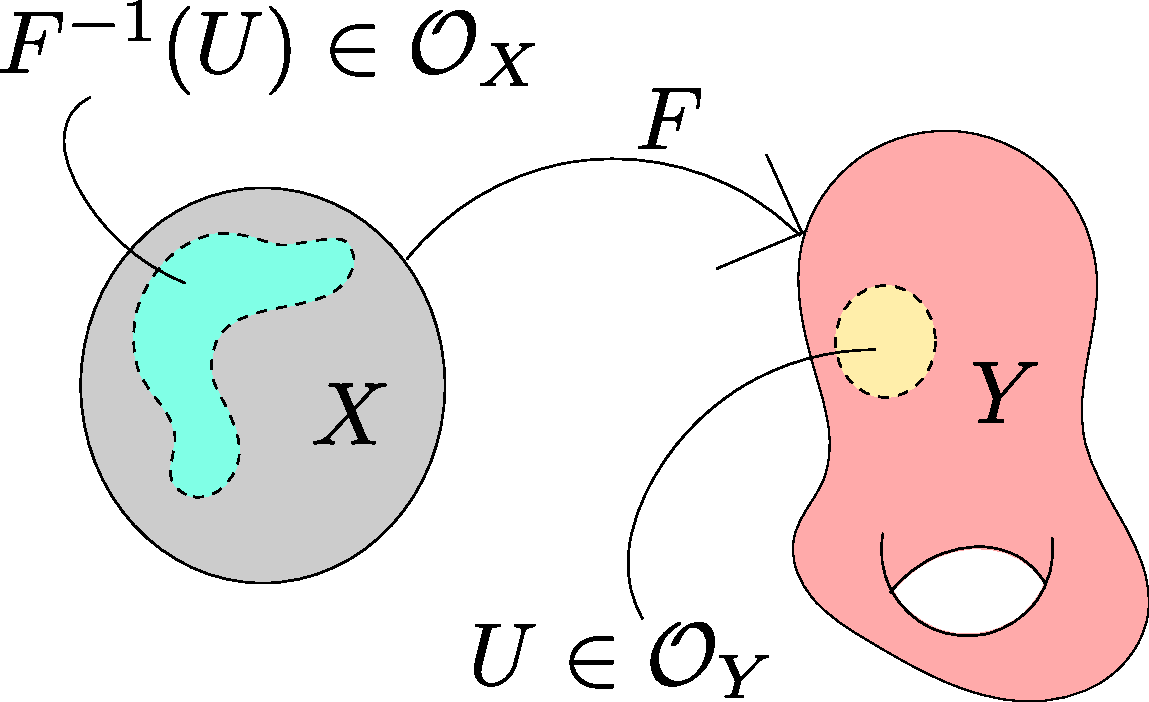
\includegraphics[width=0.8\textwidth]{images/stetigeAbb.pdf}
\caption{Stetige Abbildung}
\end{figure}

\begin{remark}
Ist $(X,d)$ ein metrischer Raum, so sind die offenen Mengen der von der Metrik induzierten Topologie Vereinigungen von endlichen Durchschnitten von Umgebungen
$U_{\epsilon}(x):=\{y \in X \mid d (x,y) < \epsilon \} (\epsilon > 0)$, 
und $F \colon (X,d) \rightarrow (Y,d')$ ist stetig im obigen Sinn genau dann, falls für alle $\epsilon > 0$ ein $\delta > 0$ existiert mit $F(U_\delta (x)) \subset U_\epsilon (F(x))$.
\end{remark}

%\begin{Kasten}[Homotopie]
\begin{Kasten}{Homotopie}
Eine \underline{Homotopie} $H \colon f \simeq g$ zwischen zwei (stetigen) Abbildungen $f,g \colon X \rightarrow Y$ ist eine (stetige) Abbildung $$H \colon X \times I \footnote{$I = [0,1] \subset \R$} \rightarrow Y, (x,t) \mapsto H(x,t)$$ mit $H(x,0) = f(x) \text{ und } H(x,1) = g(x) \forall x \in X$.
%\end{Kasten}
\end{Kasten}


\begin{figure}[h]
\centering
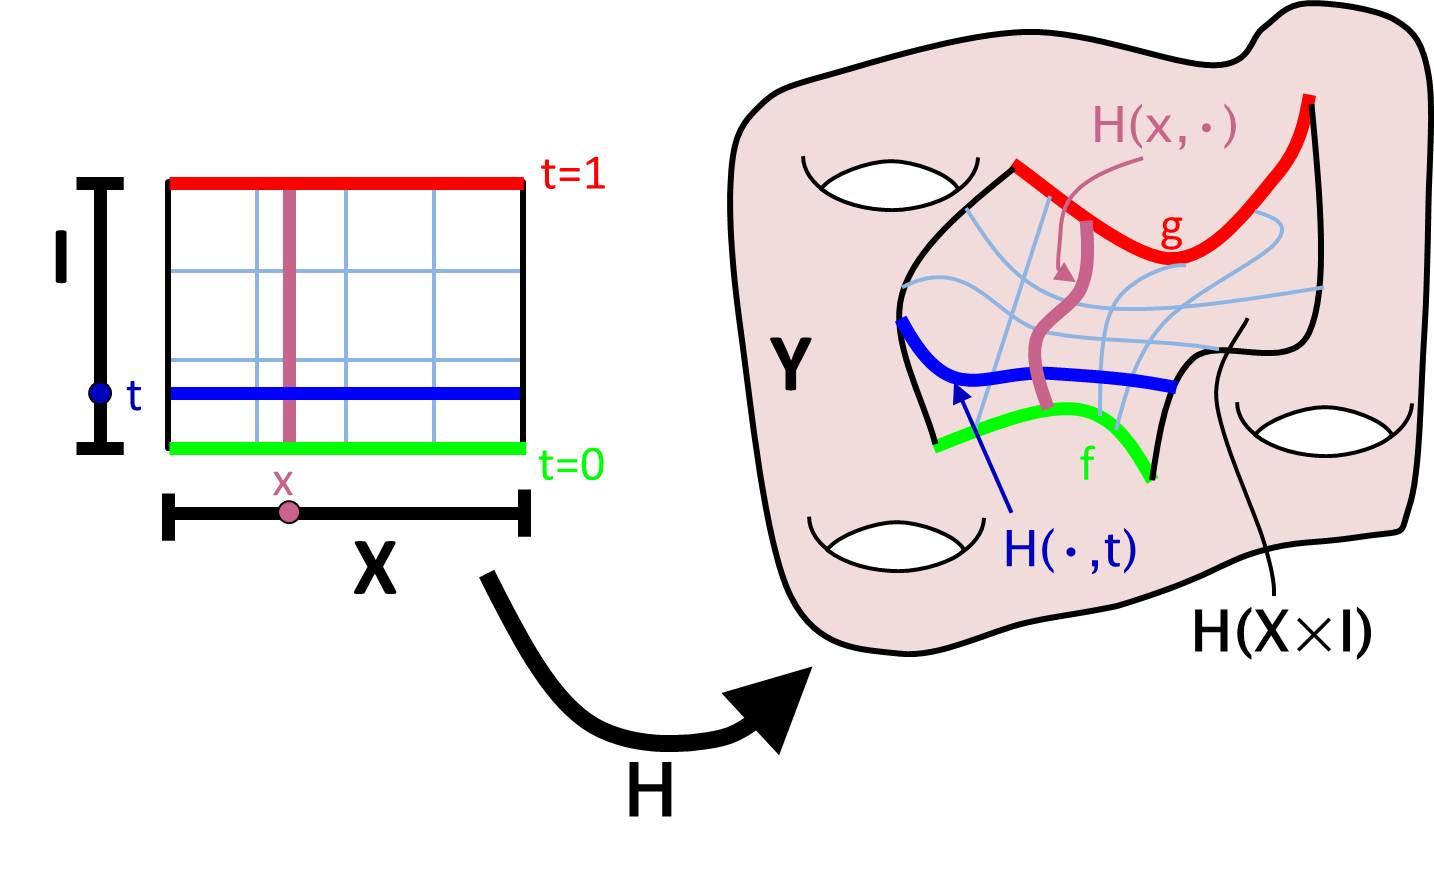
\includegraphics[width=0.7\textwidth]{images/Homotopie.jpg}
\caption{Homotopie}
\end{figure}

\begin{figure}[h]
\centering
\subfloat{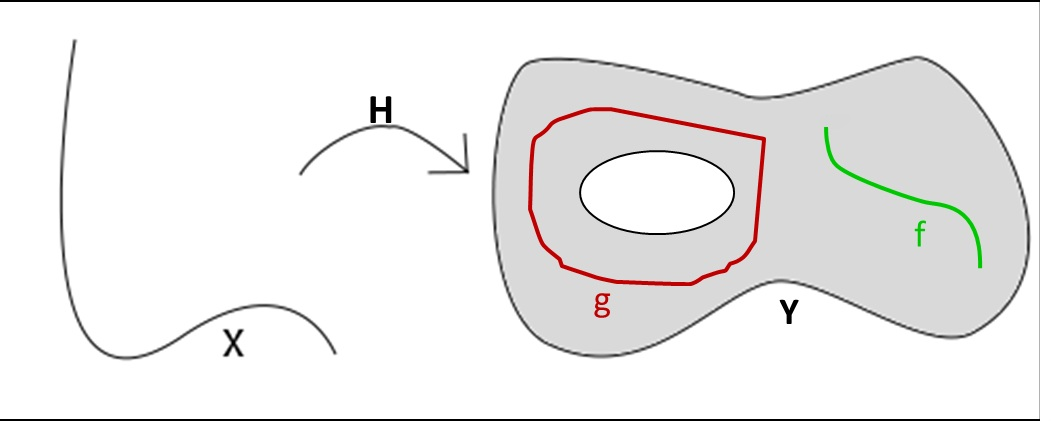
\includegraphics[width=0.5\textwidth]{images/nicht_homotop_1.jpg}}\qquad
\subfloat{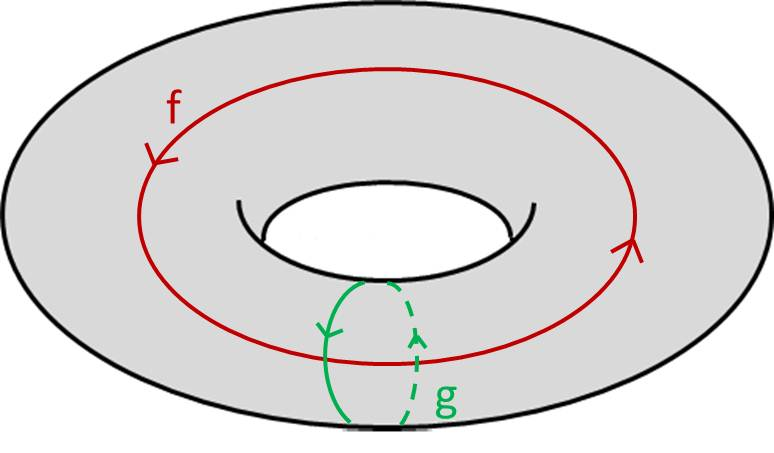
\includegraphics[width=0.4\textwidth]{images/nicht_homotop_2.jpg}}
\caption{f und g sind jeweils \underline{nicht} homotop!}
\end{figure}

\begin{remark}
$H$ heißt auch \underline{Homotopie} \underline{\underline{von $f$ nach $g$}}, eine solche ist also eine parametrisierte Schar von Abbildungen mit "Anfang" $f$ und "Ende" $g$. $f$ und $g$ heißen dann \underline{homotop}, in Zeichen: $f \simeq g$.
\end{remark}

\paragraph{Erinnerung}
Sind $X$ und $Y$ topologische Räume, so ist eine Homotopie $H = (h_t), t \in [0,1]$, eine parametrisierte Schar von stetigen Abbildungen $h_t \colon X \rightarrow Y$ mit \underline{Anfang} $h_0$ und Ende $h_1$. 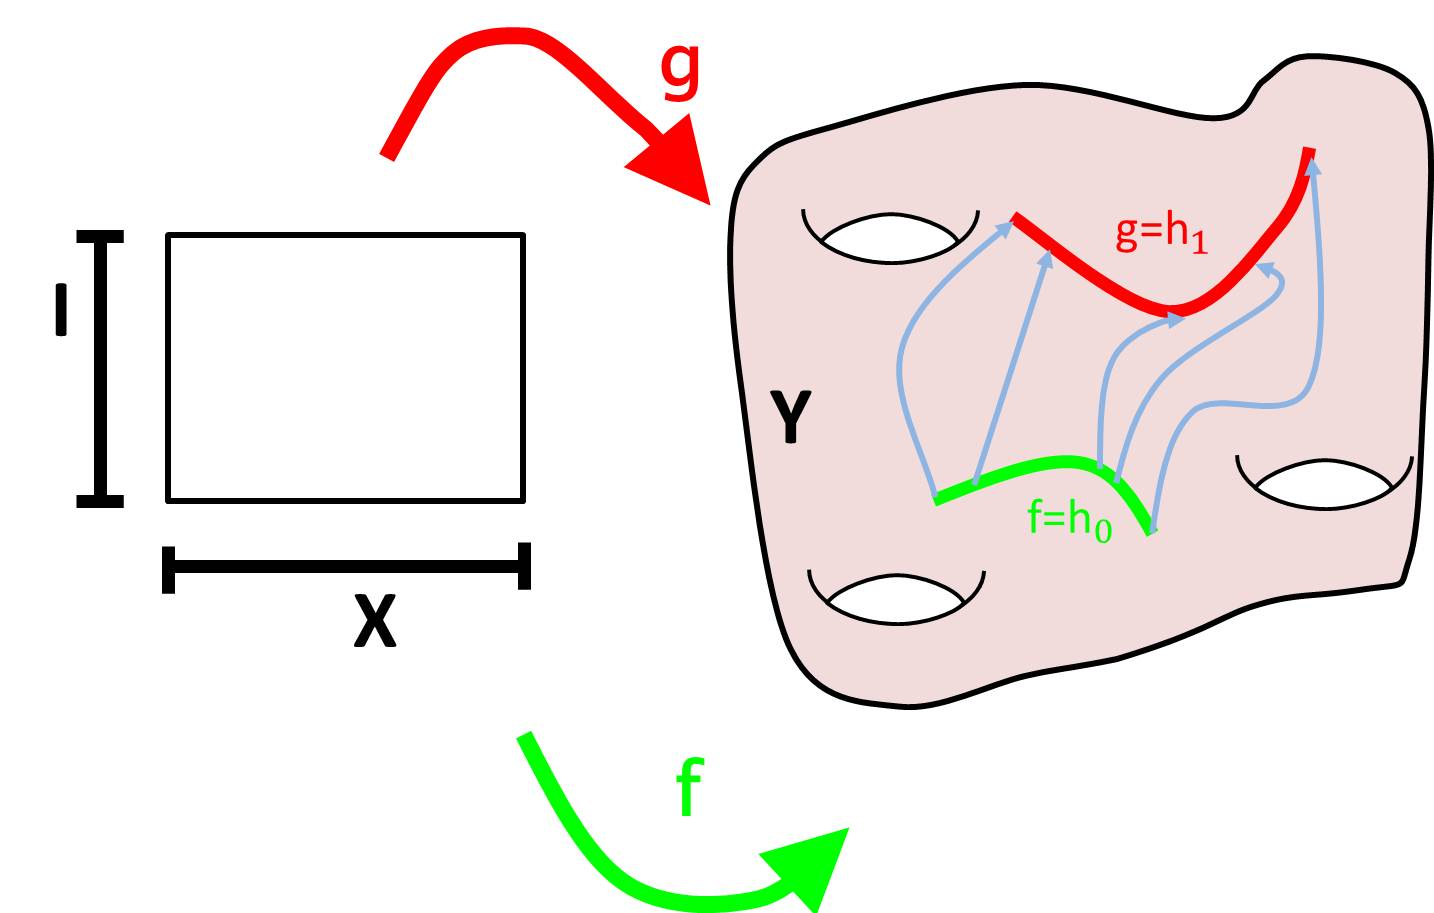
\includegraphics[width=1\textwidth]{images/Homotopie_param.jpg}

%\begin{Kasten}[homotope Abbildungen]
\begin{Kasten}{Homotope Abbildungen}
	Zwei (stetige) Abbildungen heißen \underline{homotop}, in Zeichen: $f \simeq g$, falls eine Homotopie mit Anfang $f$ und Ende $g$ existiert.
%\end{Kasten}
\end{Kasten}

\begin{remark}
"Homotop sein" ist eine Äquivalenzrelation.
\end{remark}

\begin{proof}
	\underline{Symmetrie}:
	Gilt für $f,g \in C(X,Y) := \{F \colon X \rightarrow Y \text{ stetig } \}$ $f \simeq g$ vermöge $H=(h_t), t \in [0,1],$ so liefert $(\tilde{h_t})$ mit $\tilde{h_t}:=h_{1-t}$ eine Homotopie von $g$ nach $f$, d.h. $f \simeq g \Leftrightarrow g \simeq f$.
	\newline
	\underline{Reflexivität}:
	$f \simeq f$ vermöge $h_t : \equiv f \forall t \in [0,1]$
	\newline
	\underline{Transitivität}:
	Es sei $f \simeq g$ vermöge $(h_t)$ und ferner $g \simeq l$ vermöge $(k_t)$.
	Dann liefert $M \colon X \times [0,1] \rightarrow Y$ mit
	$$M_t := \begin{cases} h_{2t} & 0 \leq t \leq \frac{1}{2} \\
	k_{2t-1} & \frac{1}{2} \leq t \leq 1
	\end{cases}$$
	eine Homotopie von $f$ nach $l$.
	\newline
	Also ist $f \simeq g, g \simeq l \Rightarrow f \simeq l$.
\end{proof}

\begin{figure}[h]
\centering
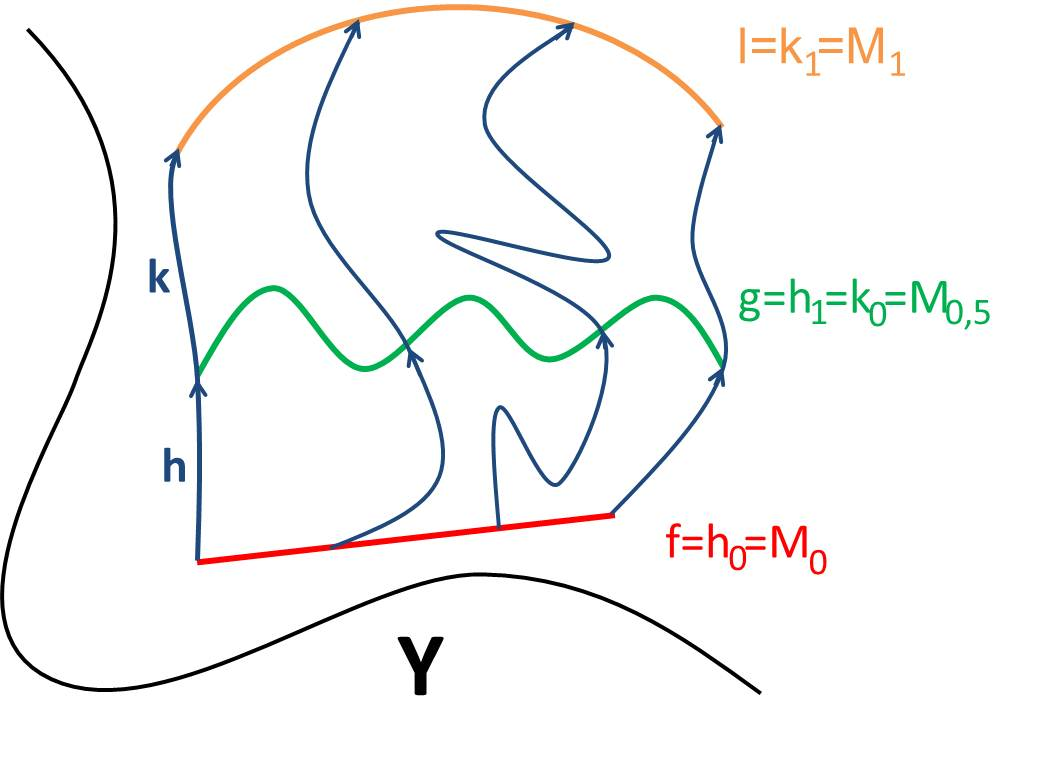
\includegraphics[width=0.8\textwidth]{images/Homotopie_Transitivitaet.jpg}
\caption{Transitivität der Relation "homotop sein"}
\end{figure}

\begin{remark}
Die Äquivalenzrelation "Homotopie von Abbildungen" liefert also eine Partition von $C(X,Y)$ in Äquivalenzklassen. Diese heißen Homotopieklassen und die \underline{Menge aller Homotopieklassen} \underline{stetiger Abbildungen} \underline{von $X$ nach $Y$} wird mit $[X,Y]$ bezeichnet.
\begin{figure}[h]
\centering
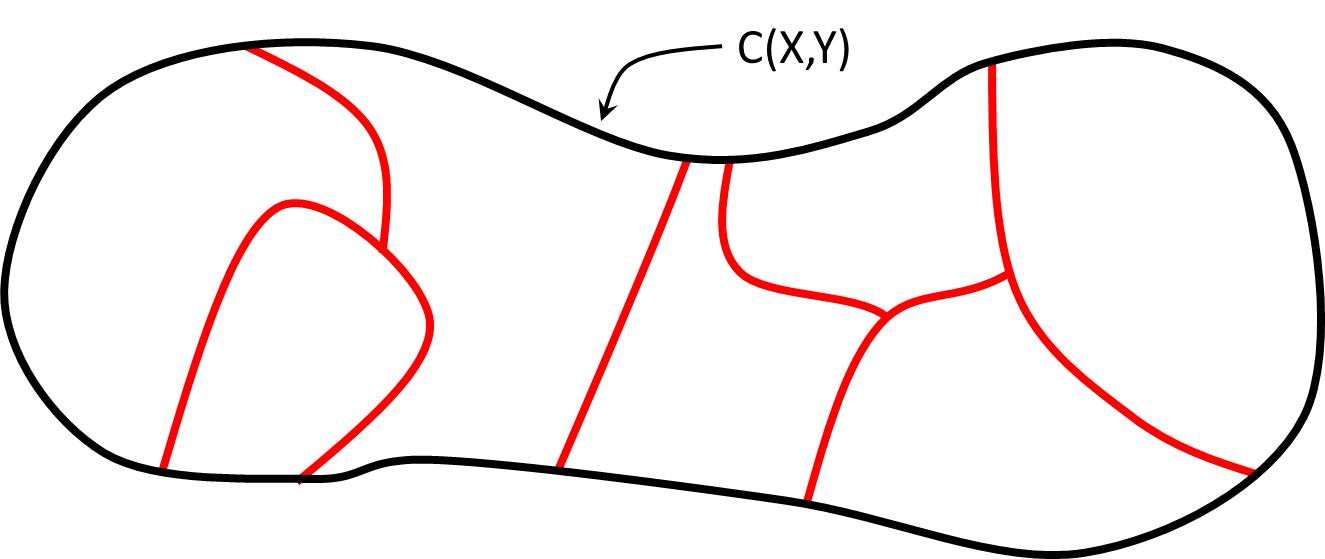
\includegraphics[width=0.8\textwidth]{images/Aequivalenzklassen.jpg}
\caption{Äquivalenzklassen $[X,Y]$ von $C(X,Y)$}
\end{figure}
\end{remark}

\begin{remark}
$C(X,Y)$ ist im Allgemeinen \underline{\underline{viel}} schwieriger zu verstehen als $[X,Y]$!
\end{remark}

\begin{example}
Je zwei stetige Abbildungen $f,g \colon X \rightarrow \R^n$ sind homotop! Denn $H(x,t):= (1-t) f(x) + t \cdot g(x)$ liefert eine Homotopie von $f$ nach $g$:
\begin{figure}[h]
\centering
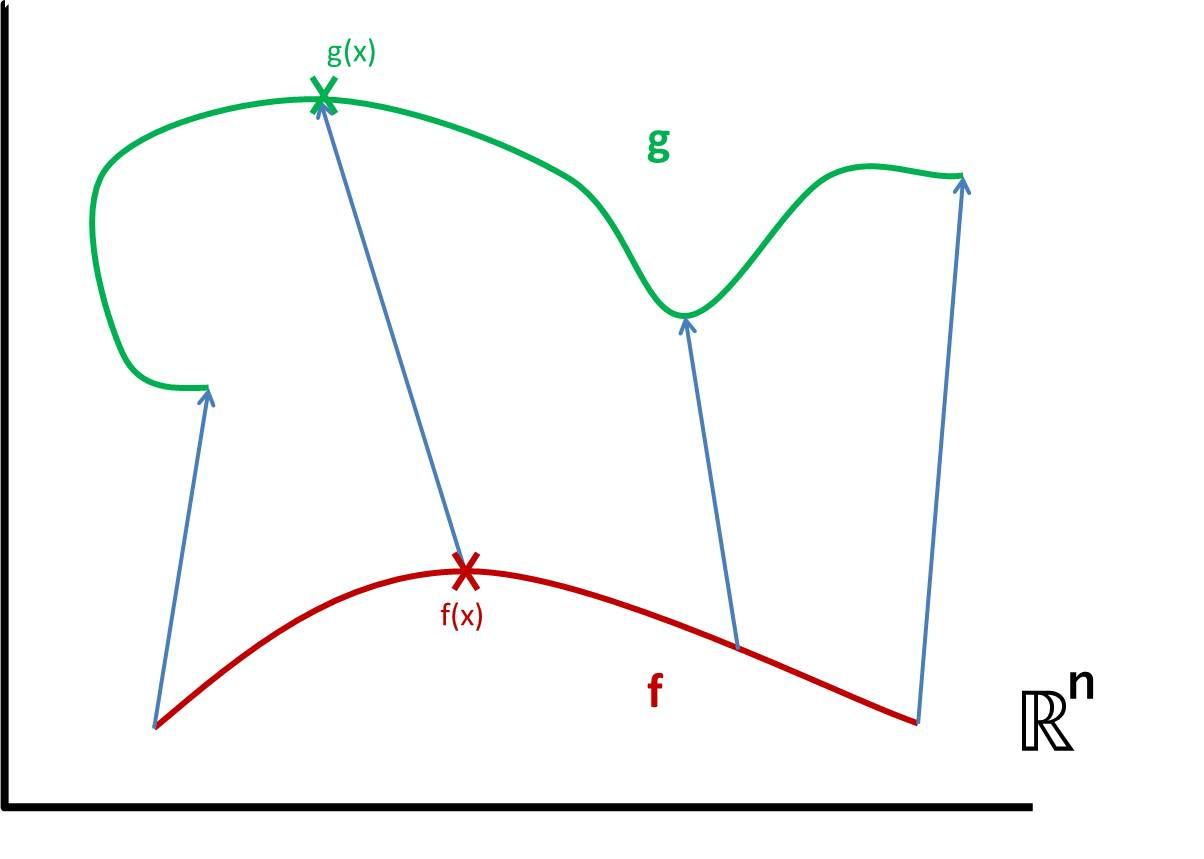
\includegraphics[width=0.8\textwidth]{images/R_n_immer_homotop.jpg}
\end{figure} 
\end{example}

%\begin{Kasten}
\begin{Kasten}{Nullhomotopie}
Eine stetige Abbildung $f \colon X \rightarrow Y$ heißt \underline{nullhomotop}, falls sie homotop zu einer konstanten Abbildung ist.
%\end{Kasten}
\end{Kasten}

\begin{figure}[h]
\centering
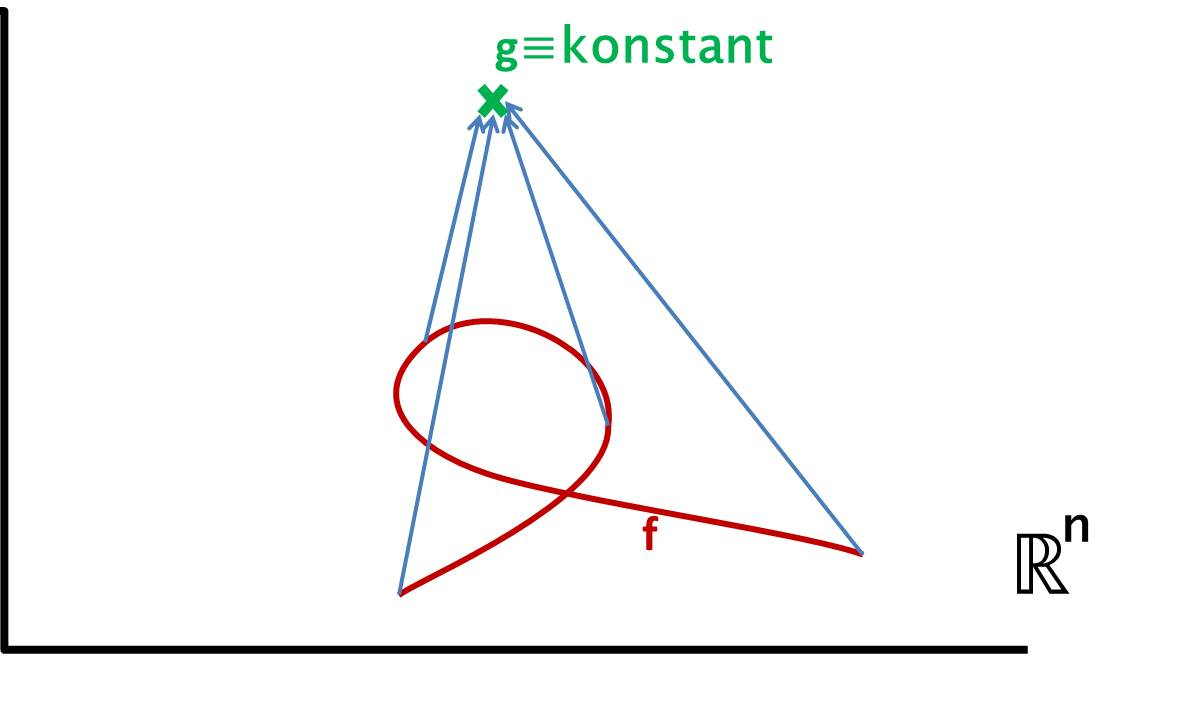
\includegraphics[width=0.8\textwidth]{images/Nullhomotopie.jpg}
\caption{f ist nullhomotop}
\end{figure}

\begin{corollary}
Jede stetige Abbildung $f \colon X \rightarrow \R^n$ ist nullhomotop, d.h. für jeden topologischen Raum $X$ besteht $[X, \R^n]$, $n$ beliebig, nur aus einem Punkt!
\end{corollary}

\begin{example}
Jeder \underline{geschlossene Weg im $\R^2$}, d.h. jede stetige Abbildung $f \colon [0,1] \rightarrow \R^2$ mit $f(0) = f(1)$ ist nullhomotop.
$\bigl[[0,1], \R^2\bigr]$ + gleicher Anfangs- und Endpunkt besteht nur aus einem Punkt, zum Beispiel der Äquivalenzklasse der konstanten Kurve $t \mapsto (1,0)$.

\begin{figure}[h!]
\centering
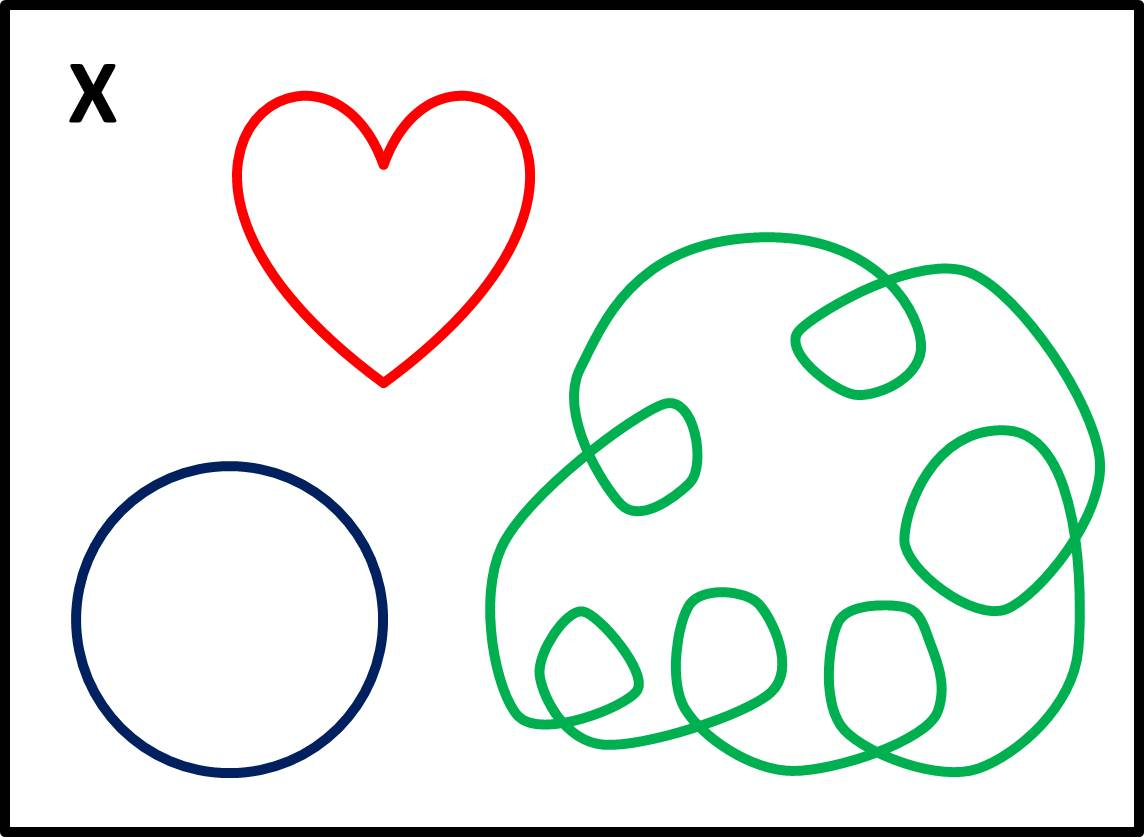
\includegraphics[width=0.8\textwidth]{images/Geschlossene_Wege.jpg}
\caption{Geschlossene Wege in $\R^n$}
\end{figure}

Interpretiere einen geschlossenen Weg im $\R^2$ auch als stetige Abbildung von $S^1 := \{ x \in \R^2 \mid \text{ } ||x|| = 1\}$ in $\R^2$, so gilt also $[S^1, \R^2]$ ist einelementig.
\newline
\underline{Aber} $[S^1, \R^2 \backslash \{0\}]$ ist nichttrivial!\newline
 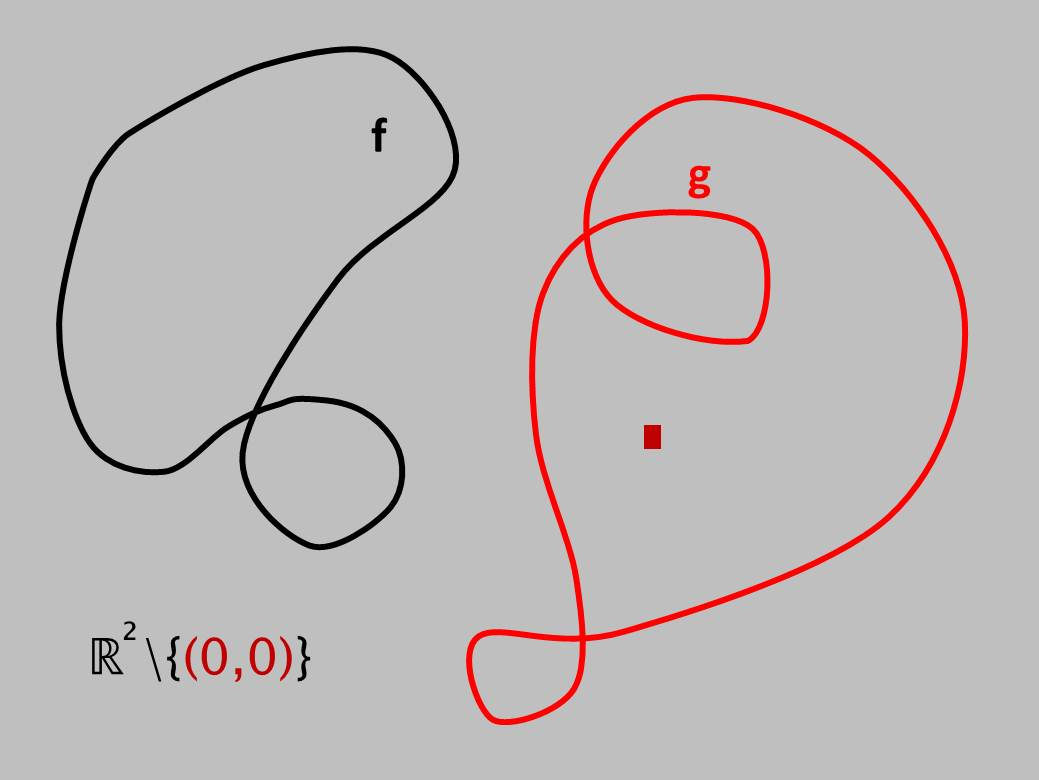
\includegraphics[scale=0.5]{images/R2_ohne_0.jpg}
\end{example}

\begin{figure}[h]
\centering
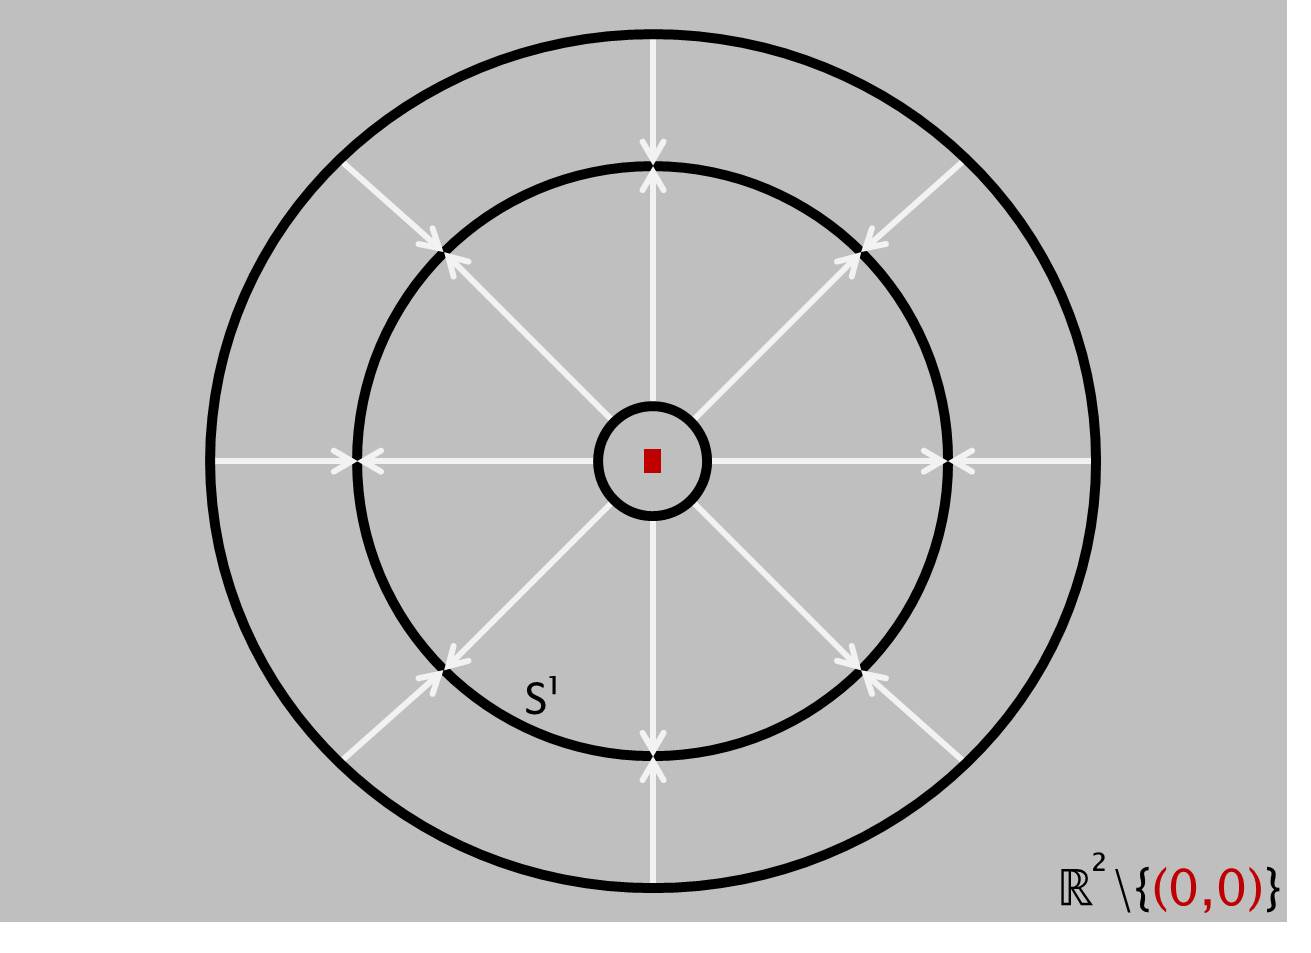
\includegraphics[width=0.8\textwidth]{images/S1_und_R2_ohne_0.jpg}
\caption{$[S^1,\R^2\backslash\{(0,0)\}]\text{ "=" }[S^1,S^1]$}
\end{figure}

%\begin{Kasten}
\begin{Kasten}{Teilraumtopologie}
Es sei $(X, \OO)$ topologischer Raum und $A \subset X$. Die auf $A$ durch
$$\OO \Big |_{A} := \{U \cap A \mid U \in \OO \}$$
induzierte Topologie heißt \underline{Teilraumtopologie} und der dadurch gegebene topologische Raum $(A, \OO \Big |_{A})$ heißt \underline{Teilraum} von $(X, \OO)$.
%\end{Kasten}
\end{Kasten}

\begin{remark}
$B \subset A$ ist also genau dann \underline{offen \underline{in $A$}}, wenn $B$ der Schnitt einer \underline{in $X$} offenen Menge mit $A$ ist.
\end{remark}

\begin{example}
$X = \R^2, A = S^1 = \{ x \in \R^2 \mid \text{ } ||x|| = 1\}$ 
\newline
\begin{figure}[h]
\centering
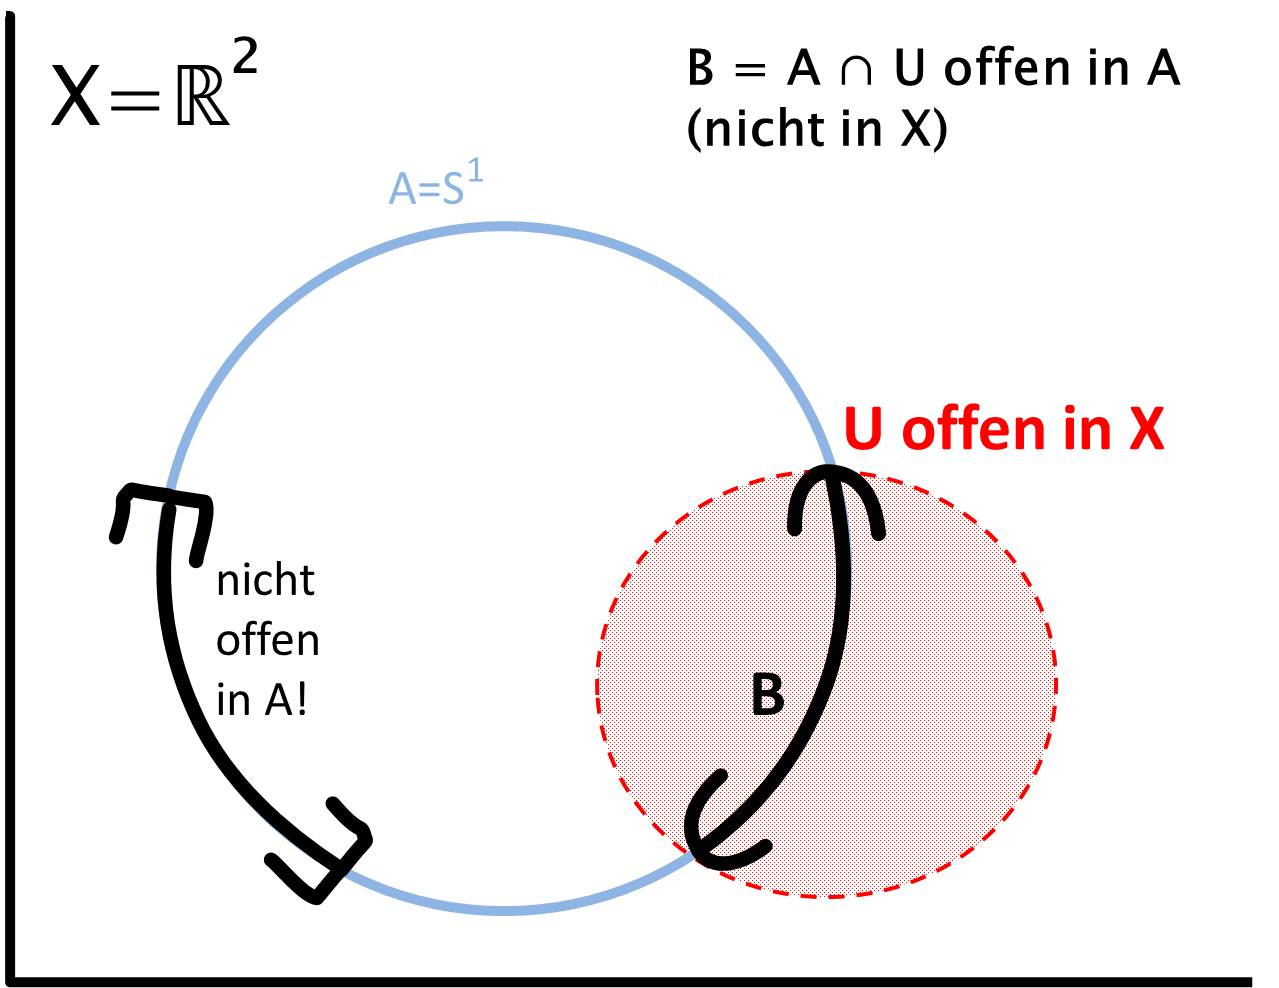
\includegraphics[width=0.8\textwidth]{images/Teilraumtopologie.jpg}
\end{figure}
\newline
\underline{Achtung:} $B$ ist \underline{\underline{nicht}} offen in $\R^2$!
\end{example}

\section{Grundlagen der allgemeinen Topologie}
\begin{example}[Beispiele topologischer Räume]
	\begin{enumerate}[(1)]
		\item $X, \OO := \{X, \emptyset\}$ \underline{`triviale Topologie'}
		\item $X, \OO := \mathcal{P}(X)$ \underline{`diskrete Topologie'}
		\item Metrische Räume, siehe unten
		\item $X:= \{a,b,c,d\} \Rightarrow \OO := \left\{X, \emptyset, \{a\}, \{b\}, \{a,c\}, \{a,b,c\}, \{a,b\} \right \}$ definiert eine Topologie auf $X$, aber $\OO^\prime:= \left \{ X, \emptyset, \{a,c,d\}, \{b,d\} \right \}$ nicht!
		\item $X := \R, \OO := \{O \mid \text{O ist Vereinigung von Intervallen } (a,b) \text{ mit } a,b \in \R\}$. $\Rightarrow (X, \OO) \text{ ist topologischer Raum}$, und $\OO$ heißt \underline{Standard-Topologie}.
		\item $X:= \R, \tilde{\OO} := \{O \mid O = \R \backslash E, E \subset \R \text{ endlich}\} \cup \{\emptyset\}$ ist auch eine Topologie auf $\R$, die so genannte $\mathcal{T}_1$-Topologie.
	\end{enumerate}
\end{example}

%\begin{Kasten}
\begin{Kasten}{Abgeschlossenheit}
	$A \subset X, X$ topologischer Raum, heißt \underline{abgeschlossen} $:\Leftrightarrow X \backslash A \text{ ist offen}$.
%\end{Kasten}
\end{Kasten}

\begin{remark}
	Beliebige Durchschnitte abgeschlossener Mengen sind abgeschlossen, ebenso endliche Vereinigungen und genauso $X$ und $\emptyset$.
\end{remark}

\begin{example}
	In einem diskreten topologischen Raum sind \underline{alle Teilmengen} abgeschlossen, in $\R_{\mathcal{T}_1}$\footnote{$\R$ mit $\mathcal{T}_1$-Topologie} alle endlichen Teilmengen und $X, \emptyset$.
\end{example}

%\begin{Kasten}
\begin{Kasten}{Umgebung}
	Ist $X$ topologischer Raum und $x \in X$, so heißt jede \underline{offene} Teilmenge $O \subset X$ mit $x \in O$ eine \underline{Umgebung} von $x$.
%\end{Kasten}
\end{Kasten}

\begin{remark}
	Umgebungen sind per definitionem offen! \newline
	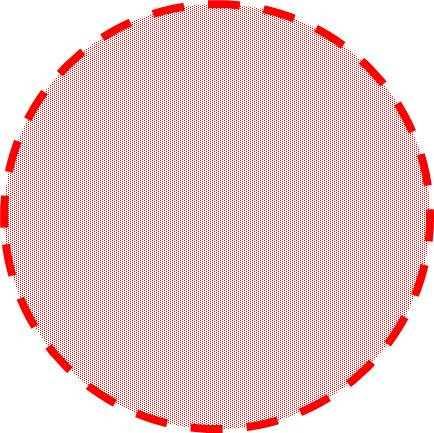
\includegraphics[scale=0.3]{images/offener_Kreis.jpg} $\qquad\qquad$ 
\includegraphics[scale=0.3]{images/offenes_Quadrat.jpg}
\end{remark}

\begin{remark}
	Jede offene Teilmenge von $\R_{Standard}$ ist eine Vereinigung disjunkter offener Intervalle, doch abgeschlossene Teilmengen von $\R$ sind keinesfalls immer Vereinigungen abgeschlossener Intervalle!
\end{remark}

\begin{example}[Die \underline{Cantor-Menge} $\mathcal{C}:= \left \{ x \in \R \mid x = \sum\limits_{k=1}^{\infty}{\frac{a_k}{3^k}}, a_k \in \{0,2\} \right \}$]
	$\Rightarrow$ $\mathcal{C}$ ist abgeschlossen in $\R$, enthält überabzählbar viele Elemente und hat `Hausdorff-Dimension' $\frac{\ln 2}{\ln 3} \approx 0,6 \ldots$
\end{example}

\begin{figure}[h]
\centering
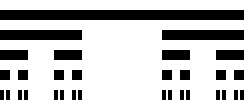
\includegraphics[width=0.8\textwidth]{images/Cantormenge_5te_Iteration.jpg}
\end{figure}

%\begin{Kasten}
\begin{Kasten}{Basis}
	Ist $(X, \OO)$ topologischer Raum mit $\mathcal{B} \subset \OO$, so heißt $\mathcal{B}$ \underline{Basis der Topologie} $:\Leftrightarrow$ Jede (nichtleere) offene Menge ist Vereinigung von Mengen aus $\mathcal{B}$.
%\end{Kasten}
\end{Kasten}

\begin{example}
	\begin{enumerate}[(1)]
		\item Die offenen Intervalle bilden eine Basis der Standard-Topologie von $\R$.
		\item Sämtliche offenen\footnote{bezüglich der euklidischen Metrik} Kreisscheiben 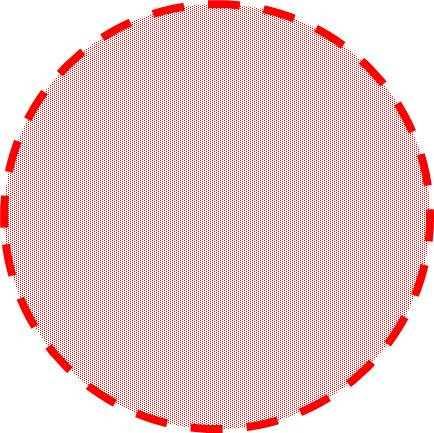
\includegraphics[scale=0.07]{images/offener_Kreis.jpg} und auch sämtliche offenen Quadrate 
\includegraphics[scale=0.07]{images/offenes_Quadrat.jpg} bilden Basen ein und derselben Topologie auf $\R^2$.
	\end{enumerate}
\end{example}

\begin{remark}
	$\bullet$ $\mathcal{B} \subset \OO$ ist Basis der Topologie von $X$ $\Leftrightarrow \forall O \in \OO \forall x \in O \exists B \in \mathcal{B} \colon x \in B \subset O$.
	\newline
	$\bullet$ $\mathcal{B} \subset \mathcal{P}(X)$ bildet die Bais \underline{einer} Topologie auf $X$ $\Leftrightarrow$ $X$ ist Vereinigung von Mengen aus $\mathcal{B}$ und der Schnitt je zweier Mengen aus $\mathcal{B}$ ist eine Vereinigung von Mengen aus $\mathcal{B}$.
	\newline
	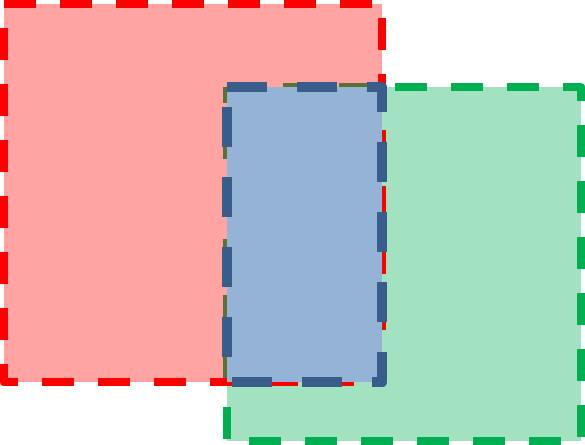
\includegraphics[scale=0.3]{images/Quadrate_Schnitt.jpg}\qquad
	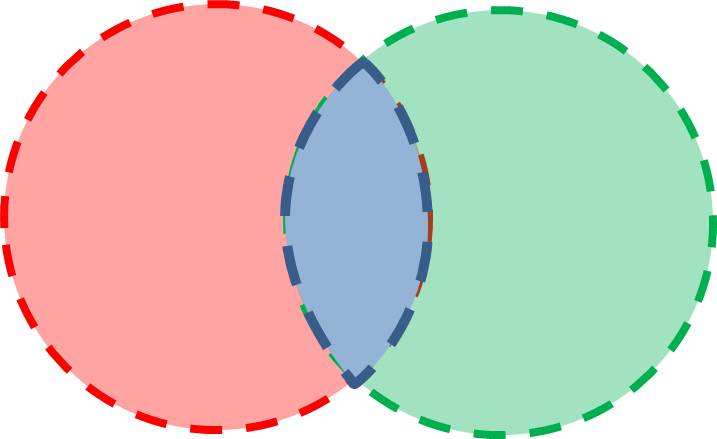
\includegraphics[scale=0.3]{images/Kreis_Schnitt.jpg}
\end{remark}

%\begin{Kasten}
\begin{Kasten}{Feiner und gröber}
	Sind $\OO_1$ und $\OO_2$ Topologien auf $X$ und $\OO_1 \subset \OO_2$, so heißt $\OO_2$ \underline{feiner} als $\OO_1$ und $\OO_1$ \underline{gröber} als $\OO_2$.
%\end{Kasten}
\end{Kasten}

\begin{example}
	$\bullet$ Die triviale Topologie ist die gröbste Topologie auf $X$, die diskrete Topologie die feinste.
	\newline
	$\bullet$ Die Standard-Topologie auf $\R$ ist feiner als die $\mathcal{T}_1$-Topologie.
\end{example}

\paragraph{Mehr zu metrischen Räumen}

%\begin{Kasten}
\begin{Kasten}{$\epsilon$-Ball, Sphäre}
	Für einen metrischen Raum $(X,d)$ und $\epsilon > 0$ sei für $p \in X$
	\begin{itemize}
		\item $B_\epsilon(p):=\{x \in C \mid d(p,x) < \epsilon \}$ der \underline{offene $\epsilon$-Ball um $p$}
		\item $D_\epsilon(p):=\{x \in C \mid d(p,x) \leq \epsilon \}$ der \underline{abgeschlossene $\epsilon$-Ball um $p$}
		\item $S_\epsilon(p):=\{x \in C \mid d(p,x) = \epsilon \}$ die \underline{ $\epsilon$-Sphäre} um $p$ (oder \underline{Sphäre vom Radius $\epsilon$})
	\end{itemize}
%\end{Kasten}
\end{Kasten}

%\begin{Kasten}
\begin{Kasten}{Metrischer Unterraum}
	Ist $(X,d)$ metrischer Raum und $A \subset X$, so heißt der metrische Raum $(A, d \big |_{A \times A})$ \underline{(metrischer) Unterraum von $X$}.
%\end{Kasten}
\end{Kasten}

\begin{example}
	Für $X=\R_{Eukl.}^{n}$ sind $B_1(0), D_1(0) =: D^n$ und $S^{n-1}:=S_1(0)$ metrische Unterräume und heißen auch offener bzw. abgeschlossener Einheitsball bzw. $(n-1)$-Sphäre.
	\newline
	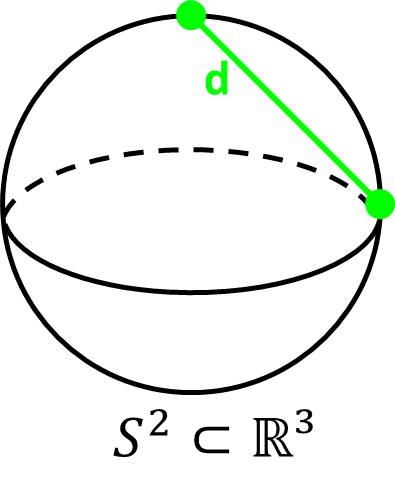
\includegraphics[width=0.3\textwidth]{images/metrischer_unterraum.jpg}
\end{example}

%\begin{Kasten}
\begin{Kasten}{Beschränktheit, Durchmesser}
	$A \subset (X,d)$ heißt \underline{beschränkt} \newline $:\Leftrightarrow \exists 0 < \rho \in \R \colon d(x,y) < \rho  \text{   } \forall x,y \in A$
	\newline
	Das Infimum, diam $A$, dieser $\rho$ heißt dann \underline{Durchmesser von $A$}.
	\newline
%\end{Kasten}
\end{Kasten}
	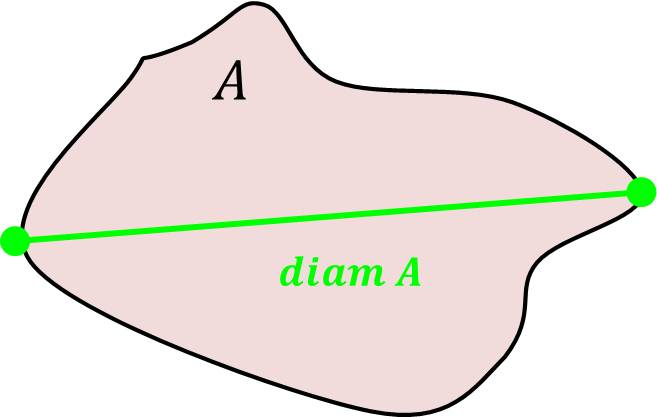
\includegraphics[width=0.4\textwidth]{images/Durchmesser.jpg}
	
\begin{remark}
	In einem metrischen Raum $(X,d)$ bilden die offenen Bälle die Basis einer Topologie $\OO=\OO_d$ von $X$, diese heißt \underline{die von der Metrik induzierte Topologie}.
\end{remark}

\begin{remark}
	$A \subset (X,d)$ ist \underline{offen}
	\newline
	$\Leftrightarrow \forall p \in A \exists \text{ ein offener Ball } B_\epsilon(p) \text{ um } p \text{ mit } B_\epsilon(p) \subset A$
	\newline
	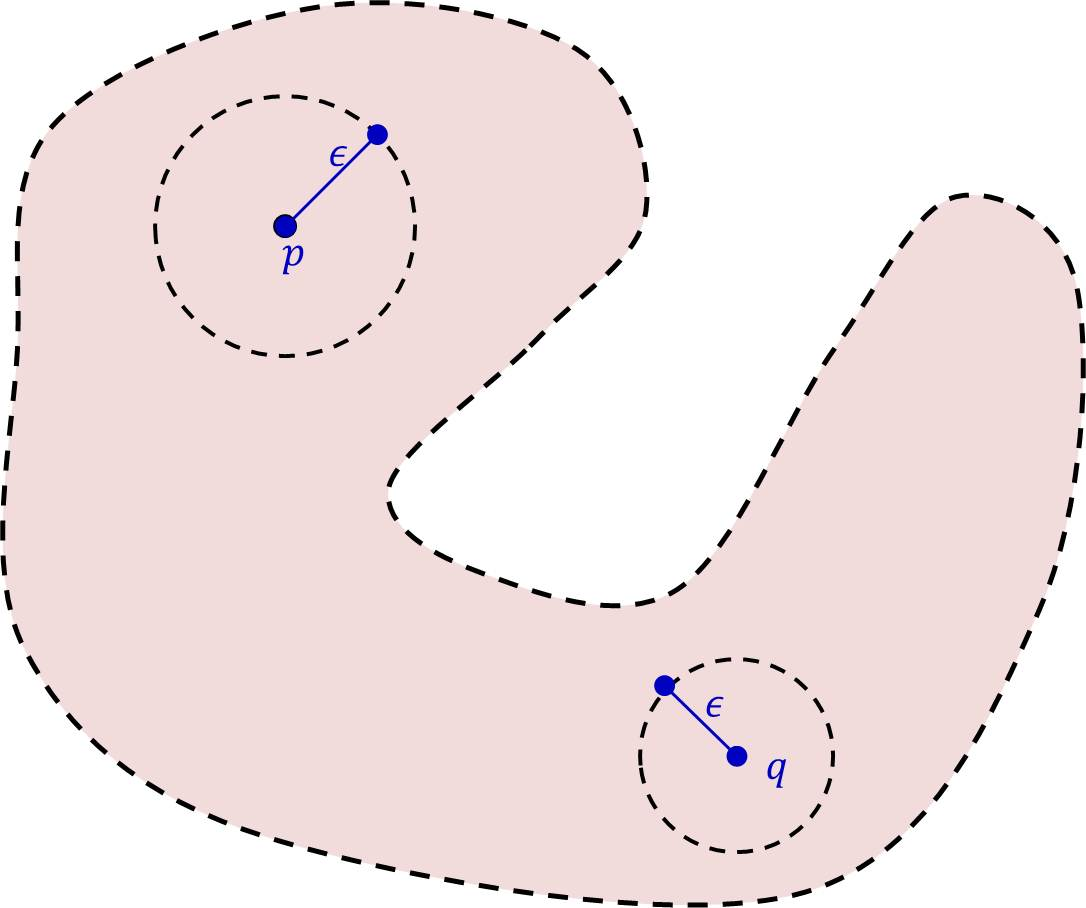
\includegraphics[width=0.6\textwidth]{images/metrisch_offen.jpg}
\end{remark}

%\begin{Kasten}
\begin{Kasten}{Abstand}
	$(X,d)$ sei metrischer Raum und $A \subset X, p \in X$.
	$$d(p,A) := dist(p,A):= \inf \{d(p,a) \mid a\in A \}$$
	heißt \underline{Abstand von $p$ und $A$}.
%\end{Kasten}
\end{Kasten}

\paragraph{Erinnerung}
Ist $(X, \OO)$ topologischer Raum und $A \subset X$, so definiert
$\OO_A := \{ A \cap O \mid O \in \OO \}$ eine Topologie auf $A$, die
 \underline{Teilraumtopologie} der \underline{in A} offenen Mengen.
 
\begin{remark}
	\label{offenAbgeschlossen}
	Ist $A \subset X$ \underline{offen} \underline{\underline{in $X$}}, so ist auch jede in $A$ offene Menge offen in $X$, und abgeschlossene\footnote{in $A$} Teilmengen einer in $X$ abgeschlossenen Menge $A$ sind auch abgeschlossen in $X$.
		
	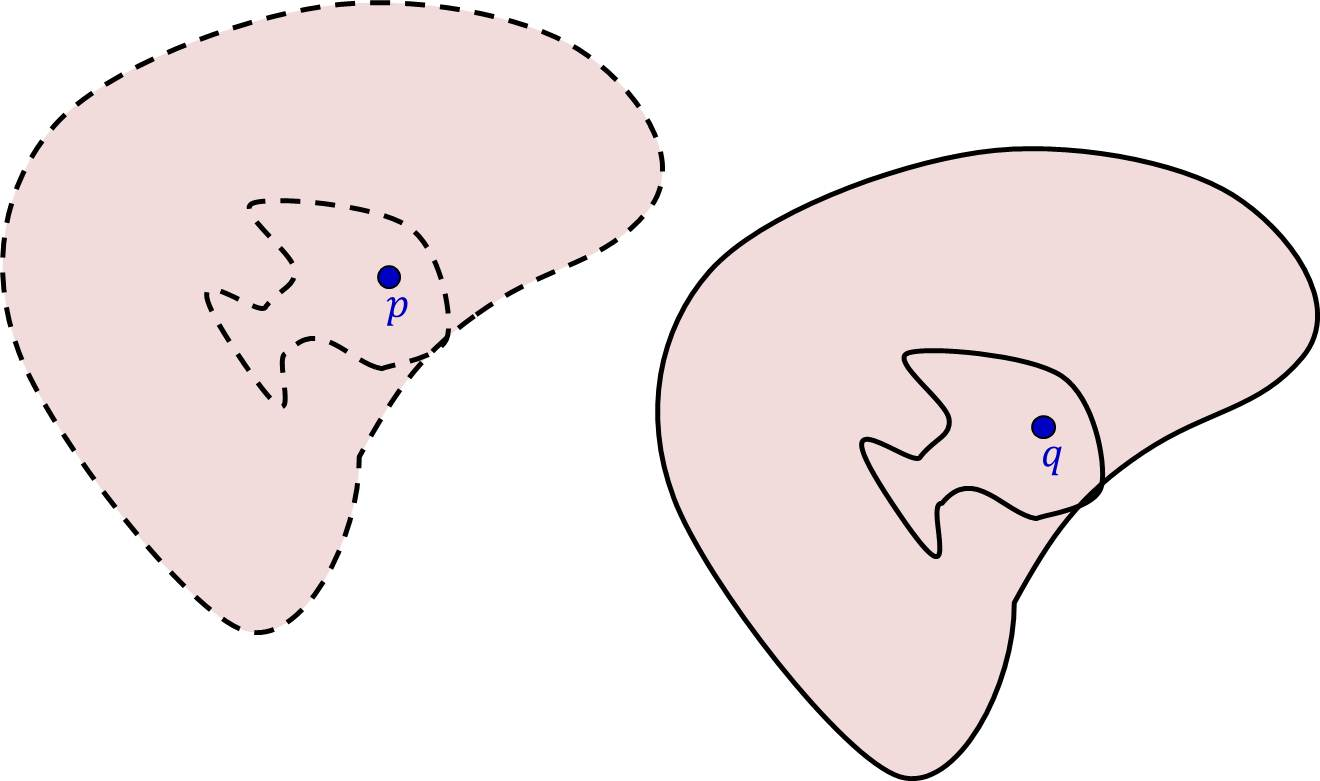
\includegraphics[width=0.6\textwidth]{images/offen_abgeschlossen.jpg}
	\newline
	Aber abgeschlossene Mengen $B$ in $A \subset X$ sind für beliebiges $A$ im Allgemeinen nicht abgeschlossen in $X$.
\end{remark}

\begin{example}[Beispiel zu Bemerkung~\ref{offenAbgeschlossen}]
	$B := A := (a,b) \subset X := \R$
\end{example}

\begin{Kasten}{Innerer Punkt, äußerer Punkt, Randpunkt}
	Für $p \in A \subset X$, $X$ topologischer Raum, heißt $p$
	\newline
	\begin{enumerate}[(1)]
		\item \underline{innerer Punkt} von $A$, falls es eine in $A$ enthaltene Umgebung $U$ um $p$ gibt. 
		\item \underline{äußerer Punkt}, falls eine zu $p$ disjunkte Umgebung $V$ in $X$ existiert.
		\item \underline{Randpunkt von $A$}, falls jede Umgebung von $p$ nichtleeren Durchschnitt mit $A$ und $X \backslash A$ hat.
	\end{enumerate}
\end{Kasten}
	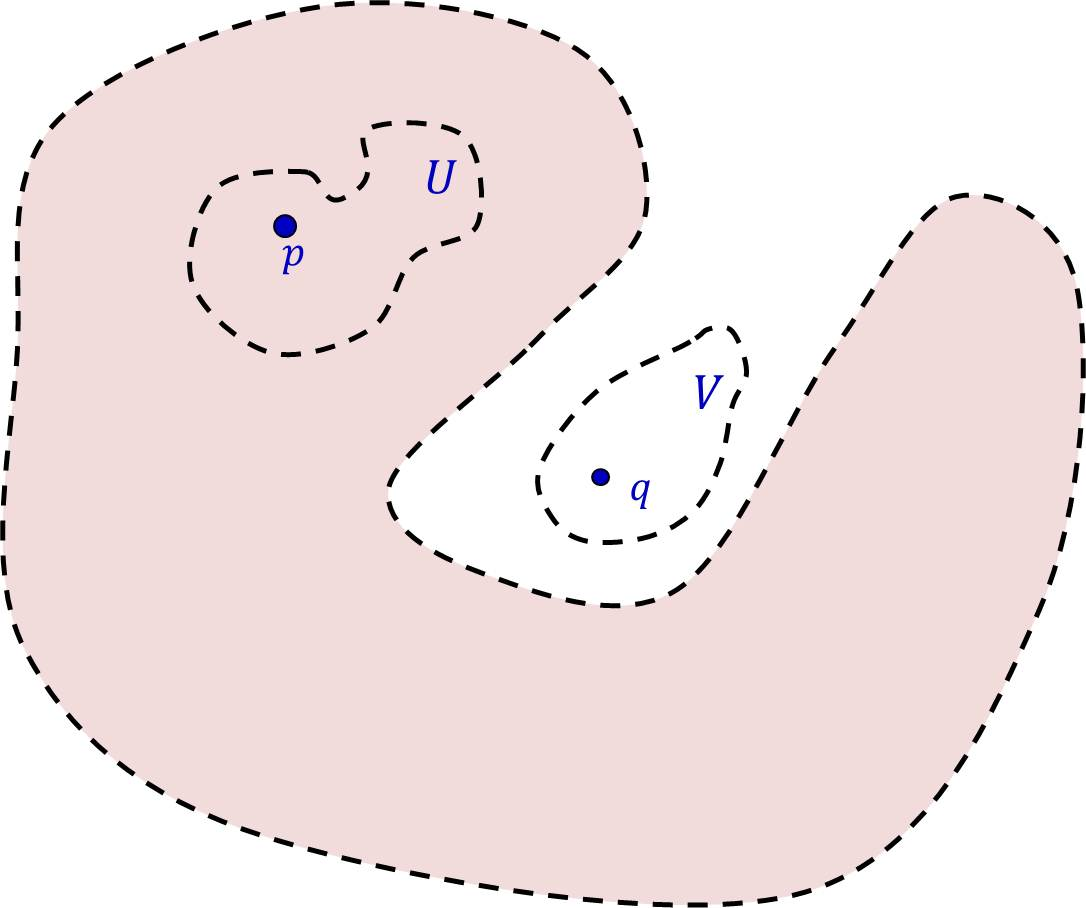
\includegraphics[width=0.6\textwidth]{images/innen_aussen.jpg}

\begin{Kasten}{Inneres}
	Für $A \subset X$ heißt die größte in $X$ offene und in $A$ enthaltene Teilmenge $\mathring A$ \underline{Inneres von $A$}.
\end{Kasten}

\begin{remark}
	$\mathring A$ ist die Menge aller inneren Punkte von $A$ und die Vereinigung aller in $X$ offenen Teilmengen von $A$, und $A \text{ ist offen } \Leftrightarrow A = \mathring A$
\end{remark}

\begin{example}
	$\mathring {\R \backslash \Q} = \mathring \Q = \emptyset$
\end{example}

\begin{Kasten}{Abschluss}
	Der \underline{Abschluss} $\bar{A}$ von $A$ ist $X \backslash \left ( \mathring {(X \backslash A} ) \right )$.
\end{Kasten}

\begin{Kasten}{Rand}
	Der \underline{Rand} $\partial A$ von $A$ ist $\partial A := \bar{A} \backslash \mathring A$, d.h. Rand $A$ = \{ Randpunkte von A \}.
\end{Kasten}

(TODO:Exkurs zu `Randbildung (topologisch) und Ableitung (analytisch) sind dual zueinander')

\begin{Kasten}{Stetigkeit}
	$f \colon X \rightarrow Y$ ist stetig $:\Leftrightarrow \forall$ offenen Mengen in $Y$ ist das Urbild unter $f$ offene Menge in $X$.
\end{Kasten}

\begin{example}
	\begin{itemize}
		\item $f \colon X \rightarrow Y$ ist stetig $\Leftrightarrow$ Urbilder abgeschlossener Mengen sind abgeschlossen.
		\item Sind $\OO_1$ und $\OO_2$ Topologien auf $X$, so ist die Identität $\text{id} \colon (X,\OO_1) \rightarrow (X,\OO_2)$ stetig $\Leftrightarrow \OO_2 \subset \OO_1$.
		\item Für $A \subset X$ ist die Teilraumtopologie $\OO_A = \OO \big |_A$ die gröbste Topologie, bezüglich der die Inklusion $i \colon A \hookrightarrow X, a \mapsto a$ stetig ist.
	\end{itemize}
\end{example}

\begin{Kasten}{Stetigkeit} %spacings stimmen nicht ganz (TODO)
	$f \colon X \rightarrow Y$ ist stetig in $x \in X$
	$:\Leftrightarrow \forall \text{ Umgebungen } V \text{ von } f(x) \exists \text{ Umgebung } U \text{ von } x \text{ mit } f(U) \subset V$.
	\newline
\end{Kasten}
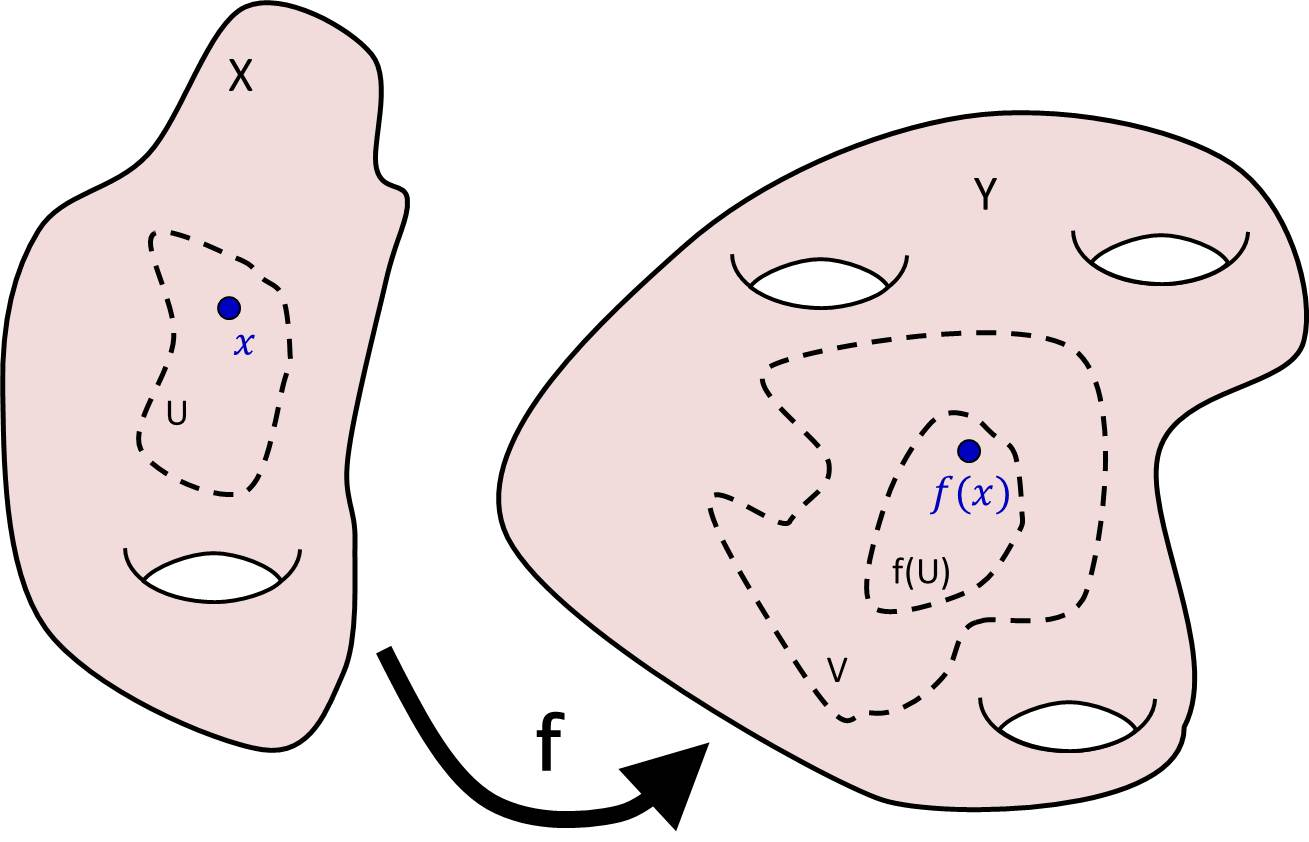
\includegraphics[width=0.7\textwidth]{images/stetig_in_x.jpg}

\begin{remark}
	$f \colon X \rightarrow Y$ ist stetig $\Leftrightarrow$ $f$ ist stetig in jedem Punkt $x \in X$.
\end{remark}

\begin{example}
	Eine Abbildung $f \colon X \rightarrow Y$ zwischen \underline{metrischen} Räumen ist bezüglich der von den Metriken induzierten Topologien stetig in $x \in X$ genau dann, wenn für jeden offenen Ball $B$ um $f(x)$ ein offener Ball um $x$ existiert, der unter $f$ in $B$ abgebildet wird. (Und ferner stetig in $x \in X$ genau dann, wenn für alle $\epsilon > 0$ ein $\delta > 0$ existiert, so dass für alle $x^\prime \in X$ mit $d_X(x,x^\prime) < \delta$ auch $d_Y \left( f(x), f(x^\prime) \right) < \epsilon$ folgt.) 
\end{example}

\begin{Kasten}{Isometrische Einbettung, Isometrie}
	Sind $X,Y$ metrische Räume, so heißt eine Abbildung $f \colon X \rightarrow Y$ \underline{isometrische Einbettung}
	\newline	
	 $: \Leftrightarrow \forall x, x^\prime \in X$ gilt $d_Y \left ( f(x), f(x^\prime) \right ) = d_X (x, x^\prime)$.
	\newline
	Eine isometrische Einbettung ist immer injektiv.
	\newline
	Ist $f$ zusätzlich \underline{bijektiv}, so heißt $f$ \underline{\underline{Isometrie}}. 
\end{Kasten}

\begin{Kasten}{Homöomorphismus}
	Eine invertierbare Abbildung $f \colon X \rightarrow Y$ topologischer Räume heißt \underline{Homöomorphismus}, falls $f$ und $f^{-1}$ stetig sind.
\end{Kasten}

\begin{example}
	\begin{itemize}
		\item $f \colon [0,1) \rightarrow S^1 \subset \C \hat{=} \R^2, t \mapsto e^{2 \pi i t} (= \cos {2 \pi t}, \sin {2 \pi t})$ ist stetig, injektiv, aber \underline{kein} Homöomorphismus!
		\newline
		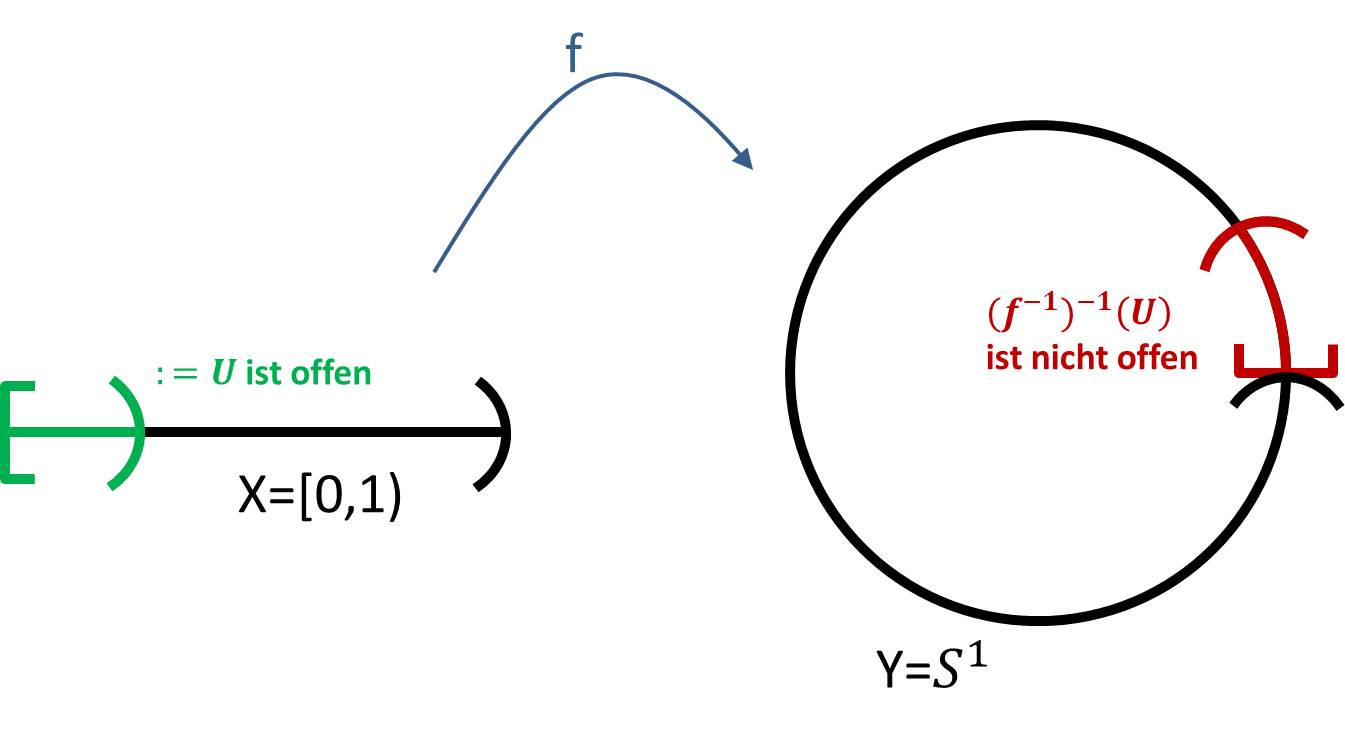
\includegraphics[width=0.7\textwidth]{images/0_1_nach_S1_f-1_nicht_stetig.jpg}
		\item $id_X \colon X \rightarrow X$ ist immer ein Homöomorphismus, Kompositionen von Homöomorphismen ebenfalls.
	\end{itemize}
\end{example}

\begin{remark}
	`Homöomorph sein' ist eine Äquivalenzrelation für topologische Räume.
\end{remark}

\begin{Kasten}{homöomorph}
	Zwei topologische Räume $X$ und $Y$ heißen \underline{homöomorph} oder \underline{vom gleichen Homöomorphietyp}, in Zeichen $X \cong Y$, falls es einen Homöomorphismus $f \colon X \rightarrow Y$ gibt.
\end{Kasten}

\begin{remark}
	Homöomorphismen erhalten sämtliche topologischen Strukturen:
	\begin{itemize}
		\item Ist $f \colon X \rightarrow Y$ Homöomorphismus, so ist $U \subset X$ offen $\Leftrightarrow f(U)$ offen in $Y$.
		\item $A \subset X$ ist abgeschlossen $\Leftrightarrow f(A)$ ist abgeschlossen in $Y$.
		\item $f(\bar{A}) = \overline{f(A)}, f(\mathring A) = \mathring{\left(f(A)\right)}$.
		\item $U$ ist Umgebung von $x \in X$ $\Leftrightarrow f(U)$ ist Umgebung von $f(x)$.
	\end{itemize}
\end{remark}

\begin{example}
	\begin{itemize}
		\item Jede Isometrie zwischen metrischen Räumen ist ein Homöomorphismus.
		\item $[0,1] \cong [a,b] \forall a < b \in \R$
		\item $(0,1) \cong (a,b) \cong \R \forall a < b \in \R$
	\end{itemize}
\end{example}

\begin{example}{Stereographische Projektion}\newline
	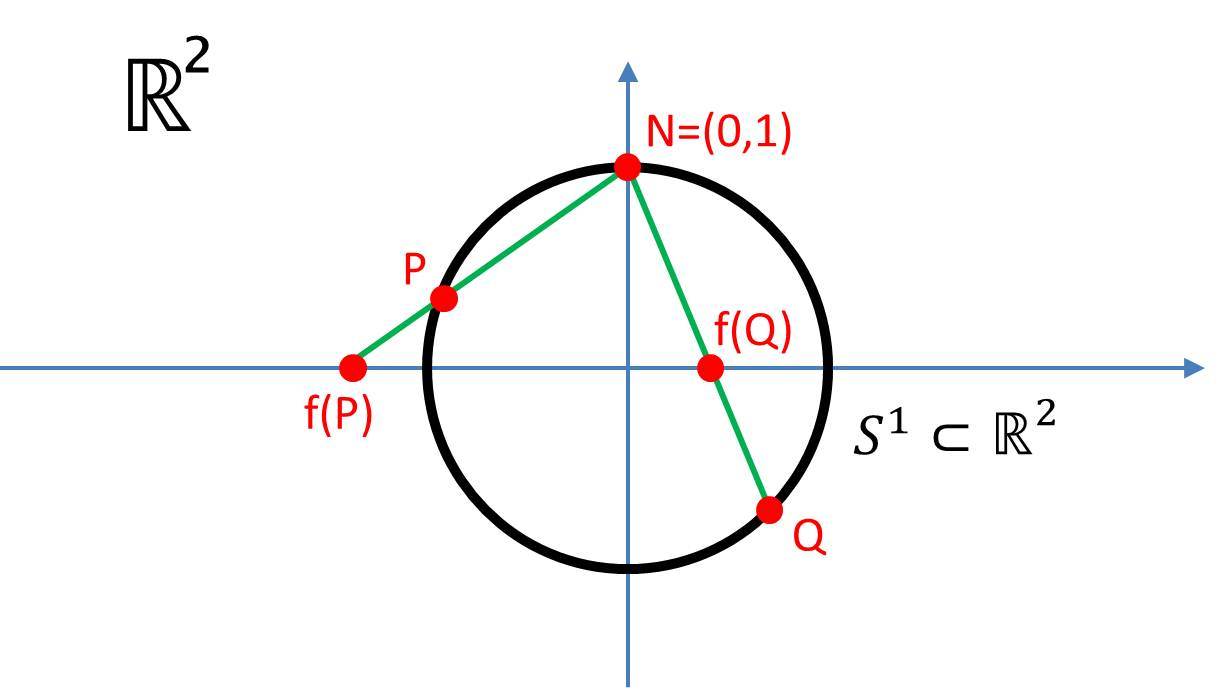
\includegraphics[scale=0.35]{images/Stereographie_S1_R1.jpg}
	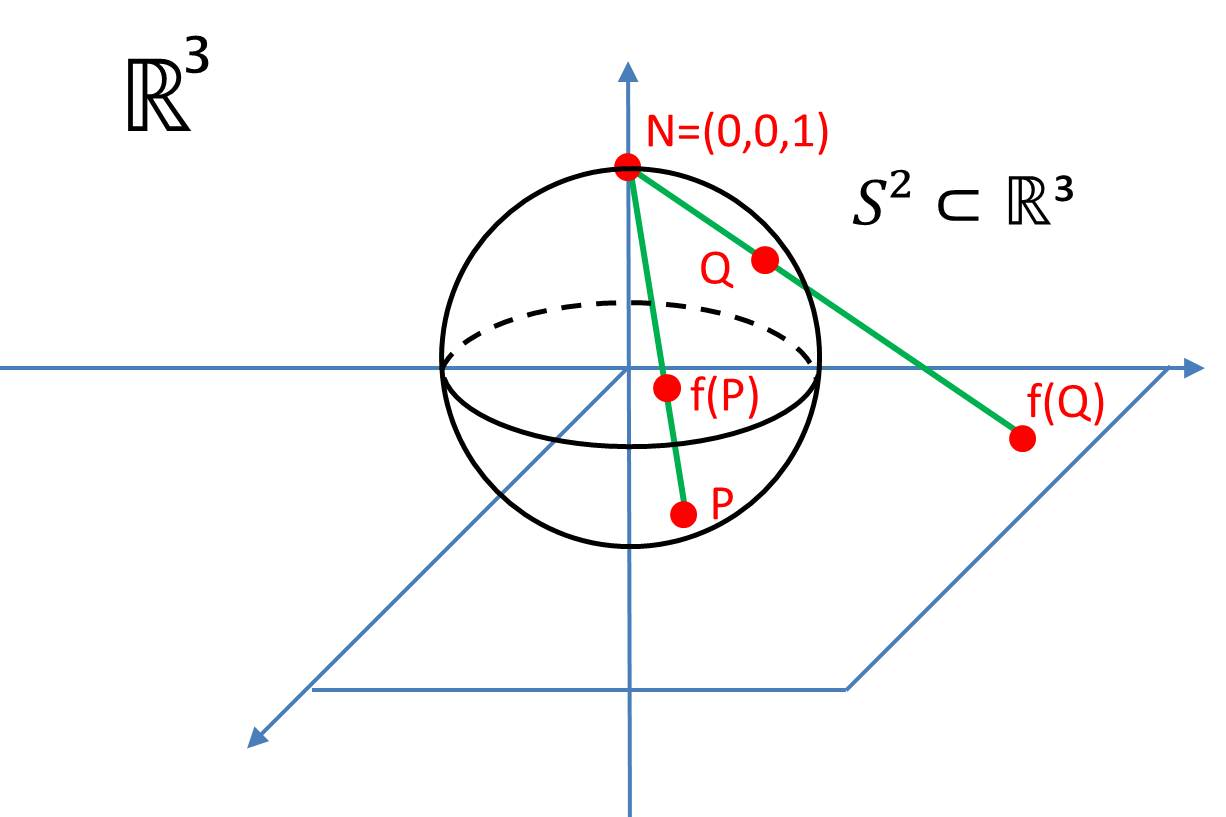
\includegraphics[scale=0.35]{images/Stereographie_S2_R2.jpg}
	\newline
	Die stereographische Projektion ist ein Homöomorphismus von $S^n \backslash \{N\}, N := (0, \ldots, 0, 1) \in \R^{n+1}$, gegeben wie folgt:
	\newline
	Der Schnitt der Geraden im $\R^{n+1}$ durch $N$ und $x \in S^n \backslash \{N\}$ mit der Hyperebene $\R^n=\{x \in \R^{n+1} \mid x_{n+1} = 0 \}$, $f(x)$, ist gegeben durch $x = (x_1, \ldots, x_{n+1}) \mapsto (\frac{x_1}{1-x_{n+1}}, \frac{x_2}{1-x_{n+1}}, \ldots, \frac{x_n}{1-x_{n+1}}) =: f(x)$ mit Umkehrabbildung $y = (y_1, \ldots, y_n) \mapsto (\frac{2 y_1}{||y||^2+1}, \ldots, \frac{2 y_n}{||y||^2+1},\frac{||y||^2-1}{||y||^2+1})$.
\end{example}

\begin{Kasten}{Einbettung}
	$f \colon X \rightarrow Y$ stetig heißt \underline{Einbettung} $:\Leftrightarrow X \overset{f}{\rightarrow}f(X) \subset Y$ Homöomorphismus.
\end{Kasten}

\begin{example}
	\begin{itemize}
		\item Für $A \subset X$ ist die Inklusion $\iota \colon A \hookrightarrow X, x \mapsto x$, stets eine Einbettung.
		\item $[0,1) \rightarrow S^1$ ist \underline{keine} Einbettung! \newline
		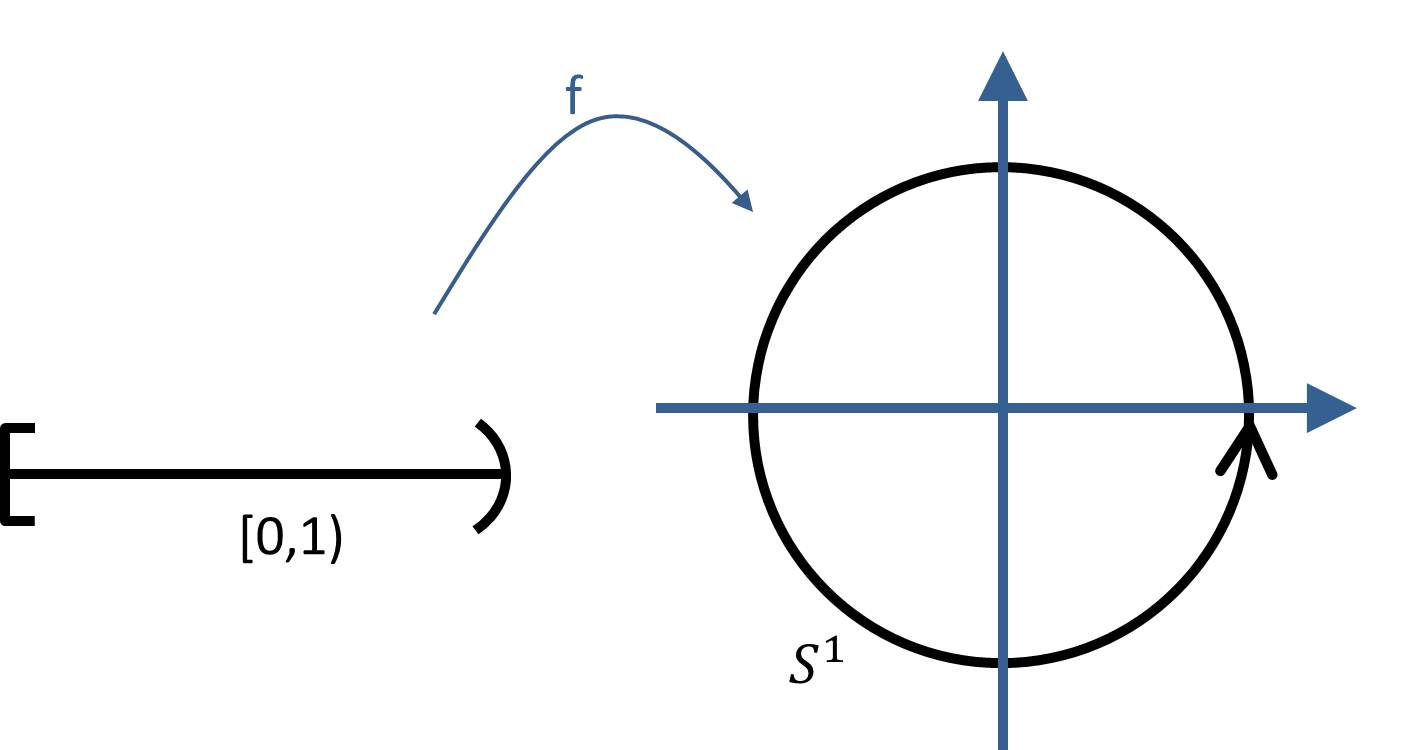
\includegraphics[scale=0.25]{images/0_1_nach_S1_Pfeil.jpg}
		\item \underline{Der Satz über die Umkehrabbildung/ Impliziter Funktionensatz} aus der Analysis zeigt: 
			\newline
			Ist $f \colon \R^n \rightarrow \R^n$ stetig differenzierbar und in $p \in \R^n$ die Jacobi-Matrix $Df(p)$ invertierbar, so existiert eine Umgebung von $p$, auf der $f \big |_U$ eine Einbettung ist.
	\end{itemize}
\end{example}

\begin{Kasten}{Äquivalenz von Einbettungen}
	Zwei Einbettungen $f,g \colon X \rightarrow Y$ heißen \underline{äquivalent} $:\Leftrightarrow \exists \text{ Homöomorphismen } h_X \colon X \rightarrow X, h_Y \colon Y \rightarrow Y \text{ mit } g \circ h_X = h_Y \circ f$, d.h. dass das Diagramm 
		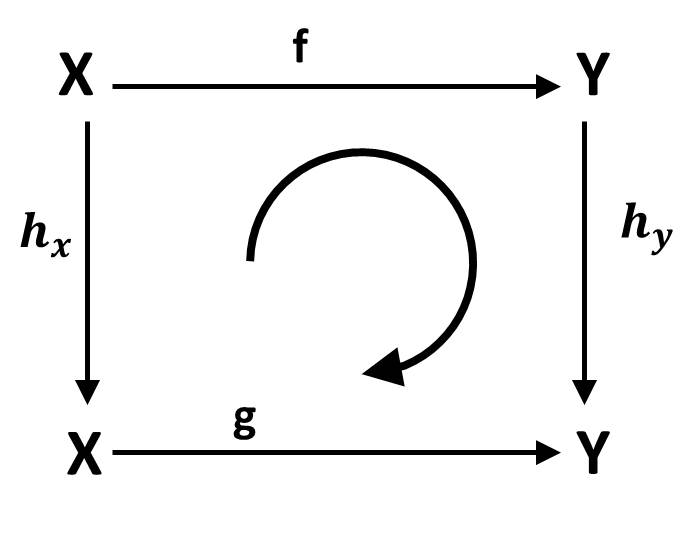
\includegraphics[scale=0.3]{images/homotopieaequivalenz.jpg} kommutiert.
\end{Kasten}

\begin{Kasten}{Knoten}
	Eine Einbettung $S^1 \rightarrow \R^3$ heißt \underline{Knoten}.
\end{Kasten}

\begin{example}
	Die Knoten mit Bildern 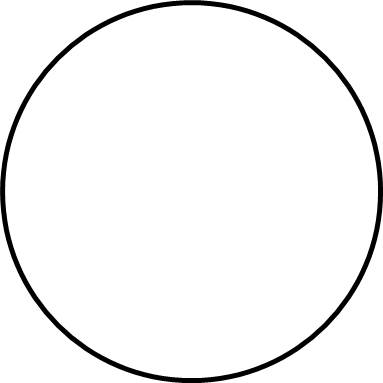
\includegraphics[scale=0.3]{images/Knoten_Kreis.jpg} und 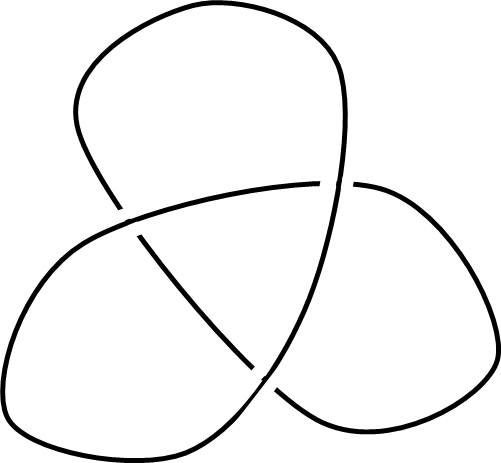
\includegraphics[scale=0.3]{images/Knoten_aequivalent_zu_Kreis.jpg} sind äquivalent, die mit 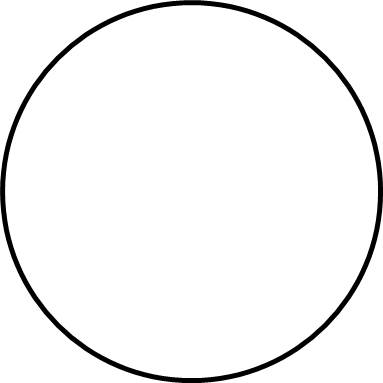
\includegraphics[scale=0.3]{images/Knoten_Kreis.jpg} und 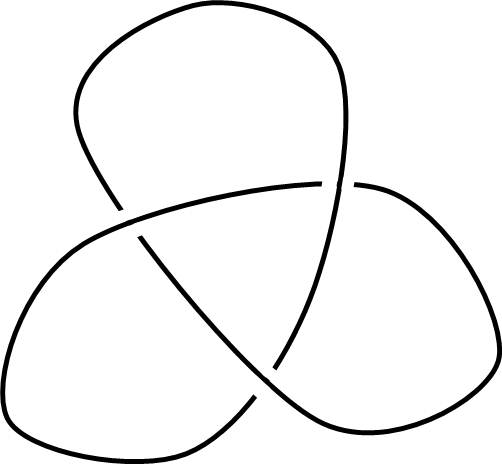
\includegraphics[scale=0.3]{images/Knoten_nicht_aequivalent_zu_Kreis.jpg} nicht!
\end{example}

\chapter{Topologische Eigenschaften}

\begin{Kasten}{zusammenhängend}
	Ein topologischer Raum heißt \underline{zusammenhängend} $:\Leftrightarrow$ Die einzigen in $X$ gleichzeitig offenen und abgeschlossenen Teilmengen sind $\emptyset$ und $X$.
	\newline
	Ansonsten heißt $X$ \underline{un-} oder \underline{nicht zusammenhängend}.
\end{Kasten}

\begin{Kasten}{Überdeckung}
	Eine Familie $\mathcal{U} = \{U_\alpha \mid \alpha \in A\}$\footnote{$A$ Indexmenge} von Teilmengen von $X$ heißt \underline{Überdeckung von $X$} $:\Leftrightarrow X = \bigcup\limits_{\alpha \in A}{U_\alpha}$.
	\newline
	$\mathcal{U}$ heißt \underline{offene} beziehungsweise \underline{abgeschlossene} Überdeckung $\Leftrightarrow$ alle $U_\alpha$ sind offen beziehungsweise abgeschlossen.
	\newline
	Für $X^\prime \subset X$ heißt eine Familie $\mathcal{U} = \{U_\alpha\}$ wie oben Überdeckung von $X^\prime$ $:\Leftrightarrow X^\prime \subset \bigcup\limits_{\alpha \in A}{U_\alpha}$.
	\newline
\end{Kasten}
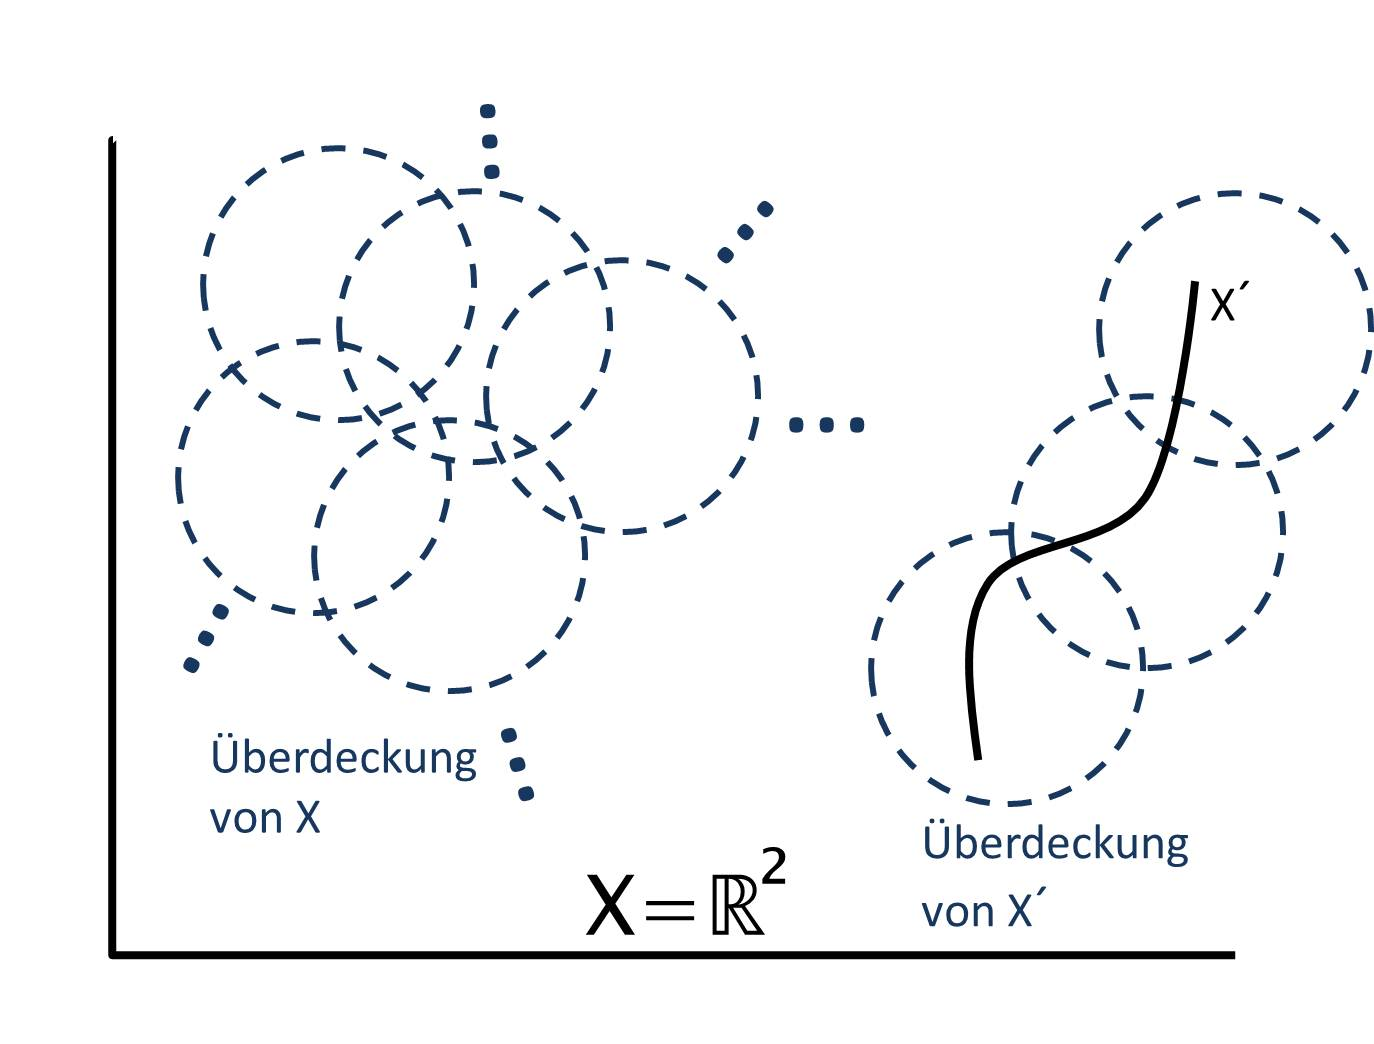
\includegraphics[scale=0.5]{images/Ueberdeckung.jpg}

\begin{Kasten}{Partition}
	Eine \underline{Partition} oder \underline{Zerlegung} einer Menge ist eine Überdeckung dieser Menge durch paarweise disjunkte Teilmengen.
	\newline
\end{Kasten}
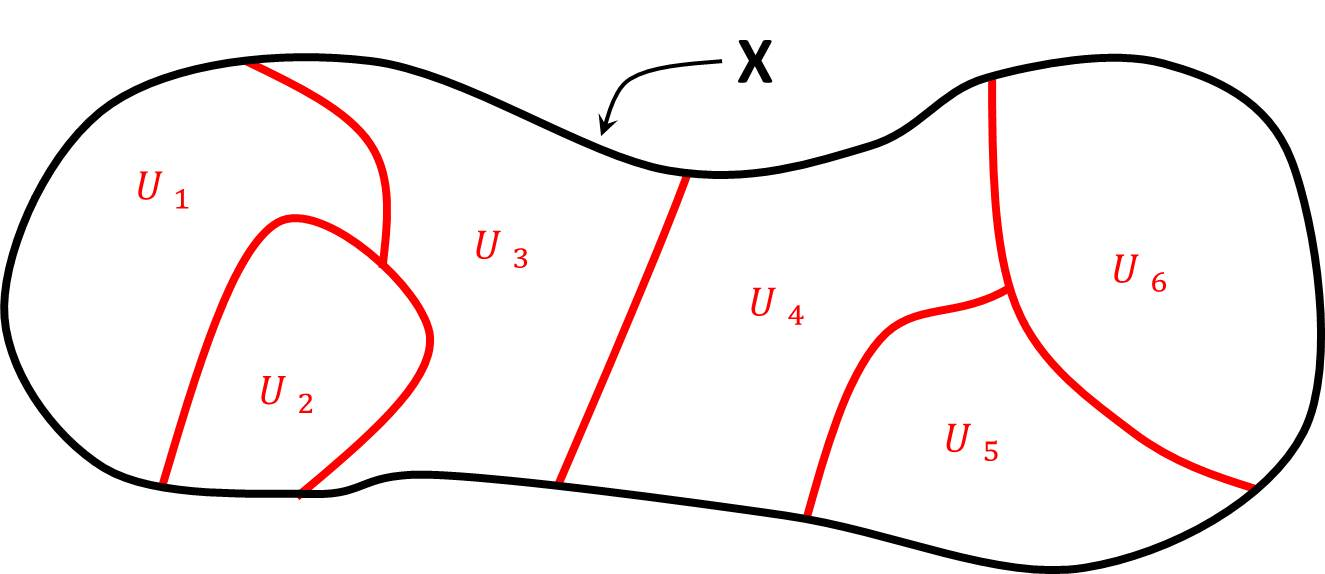
\includegraphics[scale=0.5]{images/Partition.jpg}

\begin{remark}
	Ein topologischer Raum $X$ ist zusammenhängend 
	$\Leftrightarrow$ Es existiert keine Partition von $X$ in zwei nichtleere offene Teilmengen
	$\Leftrightarrow$ es existiert keine Partition von $X$ in zwei nichtleere abgeschlossene Teilmengen
	\newline
	\underline{Denn:} $A \subset X$ ist offen \underline{und} abgeschlossen
	$\Leftrightarrow$ $A$ und $X \backslash A$ sind offen
	$\Leftrightarrow$ $A$ und $X \backslash A$ sind abgeschlossen
\end{remark}

\begin{example}
	\begin{itemize}
		\item $\Q$ als Teilmenge von $\R$ ist nicht zusammenhängend, denn $\Q = (\Q \cap (- \infty, \pi)) \cup (\Q \cap (\pi, +\infty)).$
		\item Die einzigen zusammenhängenden und mit der diskreten Topologie versehenen Räume sind $\emptyset$ und der nur aus einem Punkt bestehende Raum.
	\end{itemize}
\end{example}

\begin{remark}
	Allgemein sagt man von einer Menge, sie sei zusammenhängend, wenn diese, aufgefasst als Teilraum eines topologischen Raumes, zusammenhängend ist.
\end{remark}

\begin{example}
	$[0,1] (\subset \R)$ ist zusammenhängend, aber $[0,1] \cup (2,3)$ nicht!
\end{example}

\begin{example}
	Eine Teilmenge $A$ von $\R_{\mathcal{T}_1}$ ist zusammenhängend
	$\Leftrightarrow$ $A$ ist leer, einpunktig, oder unendlich!
\end{example}

\begin{remark}[Eigenschaften zusammenhängender Mengen]
	\begin{itemize}
		\item $A$ zusammenhängend $\Rightarrow$ $\bar{A}$ zusammenhängend
		\item $A,B \subset X$ zusammenhängend, $A \cap B \neq \emptyset \Rightarrow A \cup B$ zusammenhängend
		\item $A \cup B$ zusammenhängend, $A \cap B$ zusammenhängend $\not\Rightarrow A,B$ zusammenhängend ($A = \Q, B = \R \backslash \Q$)
	\end{itemize}
\end{remark}

\begin{Kasten}{Zusammenhangskomponente}
	Eine \underline{Zusammenhangskomponente} eines topologischen Raumes $X$ ist eine maximale zusammenhängende Teilmenge von $X$.
\end{Kasten}

\begin{remark}
	\begin{itemize}
		\item Jeder Punkt von $X$ liegt genau in einer Zusammenhangskomponente, und diese ist die Vereinigung aller diesen Punkt enthaltenden zusammenhängenden Teilmengen.
		\item Zwei Zusammenhangskomponenten sind damit entweder gleich oder disjunkt.
		\item Zusammenhangskomponenten sind abgeschlossen.
	\end{itemize}
\end{remark}

\begin{theorem}
	Stetige Bilder zusammenhängender Mengen sind zusammenhängend.
	\newline
	(D.h.: Ist $f \colon X \rightarrow Y$ stetig und $X$ zusammenhängend, so auch $f(X)\subset Y$.)
\end{theorem}

\begin{proof}
	Es sei ohne Einschränkung $Y=f(X)$ und sei $Y=U \cup V$ Partition von $Y$ in zwei offene Mengen $\Rightarrow f^{-1}(U), f^{-1}(V)$ sind offen in $X$ ($f$ stetig) und bilden eine Partition von $X$. $X$ ist zusammenhängend.
	$\Rightarrow f^{-1}(U) \text{ oder } f^{-1}(V) = \emptyset$.
	\newline
	Sei o.E. $f^{-1}(U) = \emptyset \Rightarrow U = f(\emptyset) = \emptyset \Rightarrow V = f(X)$ ($f$ surjektiv auf $f(X)$)
	\newline
	$\Rightarrow$ Es existiert \underline{keine} Partition von $Y$ in nichtleere offene Mengen $\Leftrightarrow Y$ zusammenhängend.
\end{proof}

\begin{corollary}
	Zusammenhang bleibt unter Homöomorphismen erhalten, und ebenso die Zahl der Zusammenhangskomponenten.
\end{corollary}

\begin{example}
	Für $n > 1$ sind $\R^n$ und $\R$ nicht homöomorph!
	\newline
	\underline{Denn:} $\R^n \cong \mathring{D}^n$ (Einheitskugel) und nimmt man aus $\mathring{D}^n$ einen Punkt $p$ heraus, so bleibt für $n>1$ $\mathring{D}^n \backslash \{p\}$ zusammenhängend, $\mathring{D}^1 = (-1,1) \cong \R$ aber nicht!
	\newline
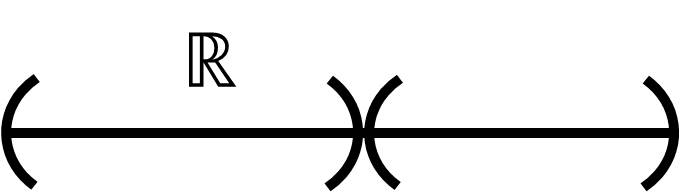
\includegraphics[scale=0.4]{images/R_ohne_p.jpg}$\qquad\qquad$
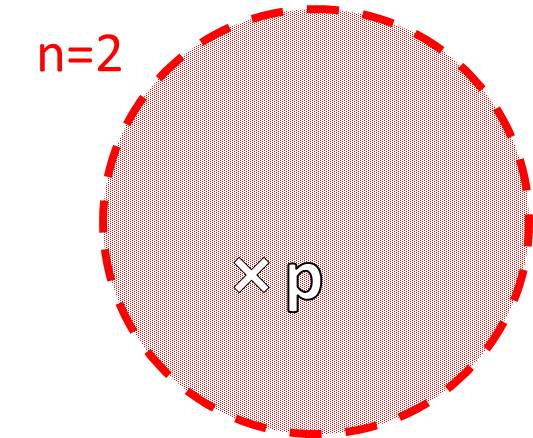
\includegraphics[scale=0.4]{images/R2_ohne_p.jpg}
	\newline
	\underline{Allgemeiner (Brouwder)} $\R^m \cong \R^n \Leftrightarrow m=n$
\end{example}

\begin{corollary}{Zwischenwertsatz:}
	Eine stetige Funktion $f \colon [a,b] \rightarrow \R$ nimmt jeden Wert zwischen $f(a)$ und $f(b)$ an.
\end{corollary}

\begin{example}{Waffel teilen.}
	Eine Waffel, wie unregelmäßig auch immer, lässt sich immer in zwei gleich große Teile schneiden.
	\newline
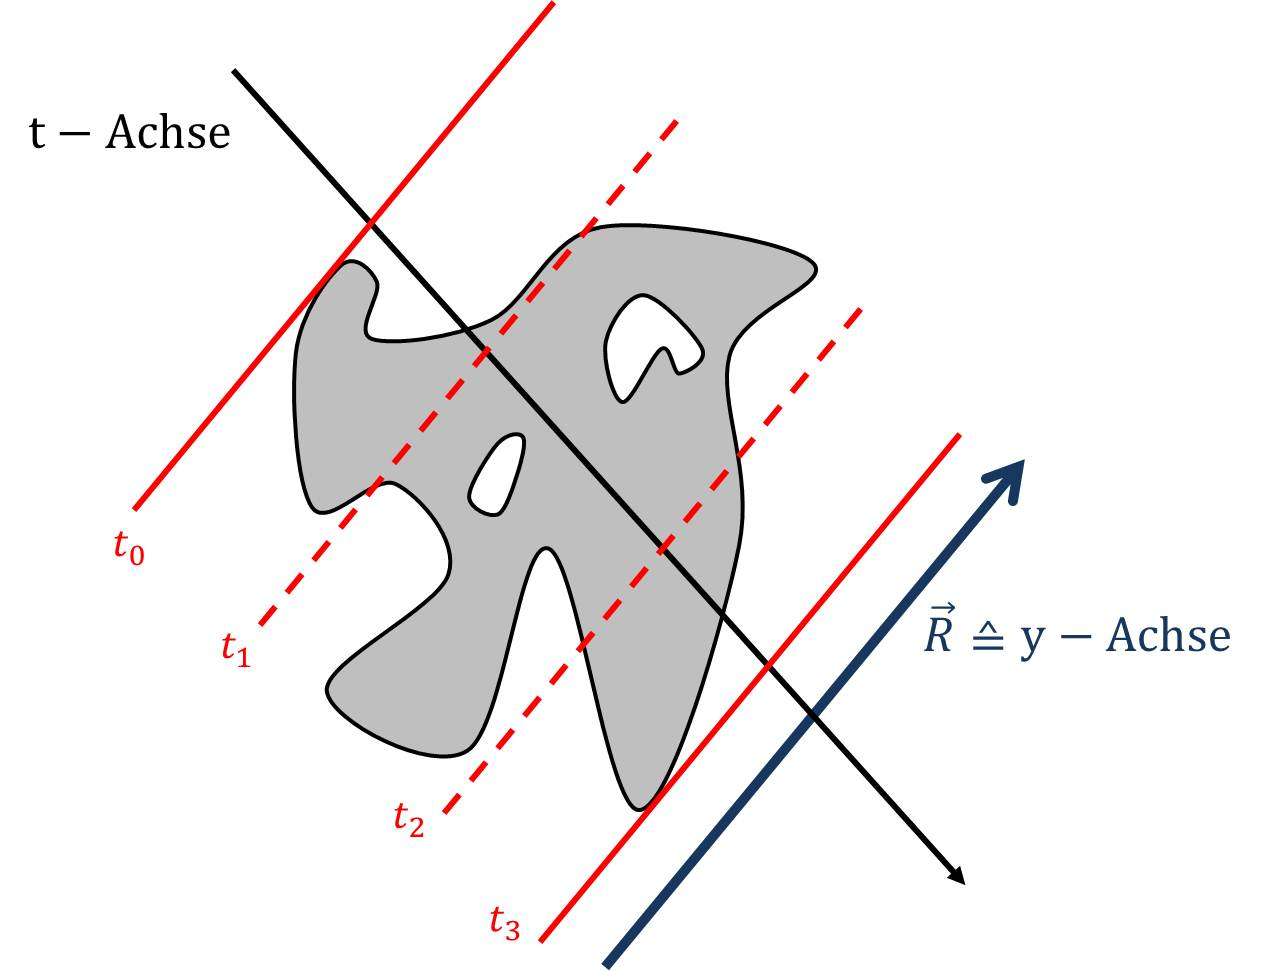
\includegraphics[scale=0.4]{images/Waffel_zshgd.jpg}
\newline
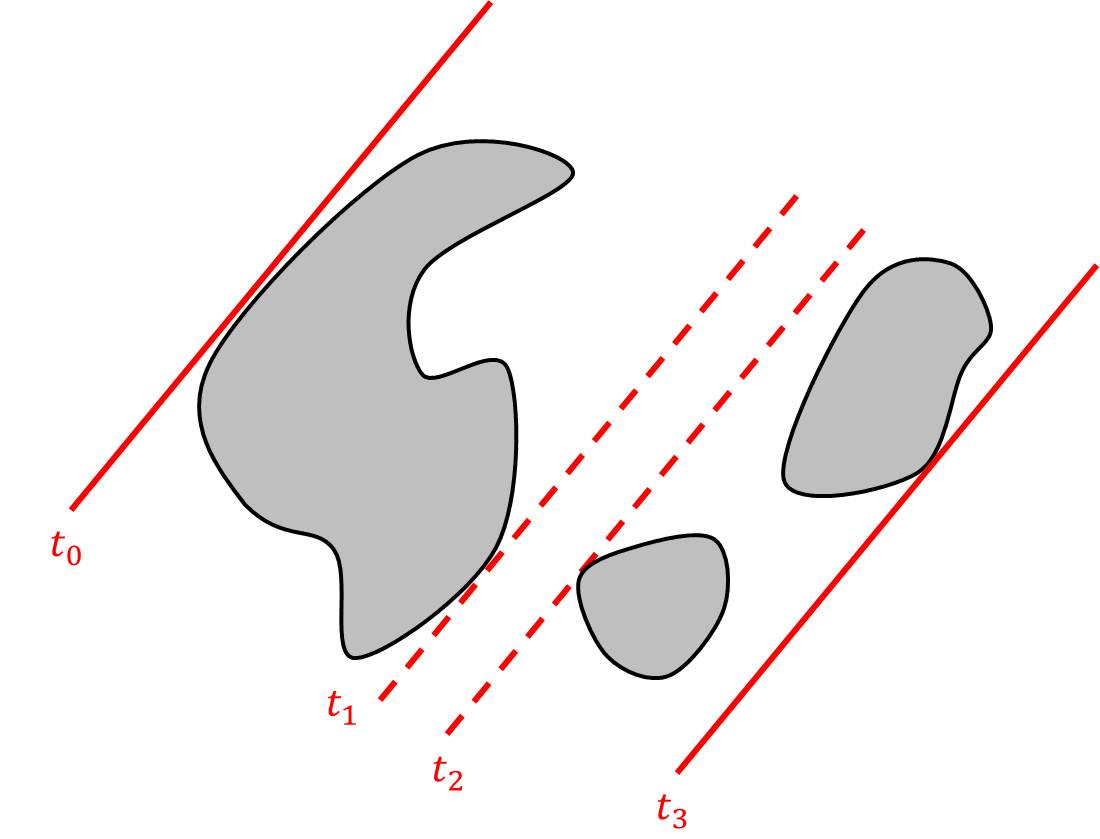
\includegraphics[scale=0.3]{images/Waffel_unzshgd.jpg} $\qquad$
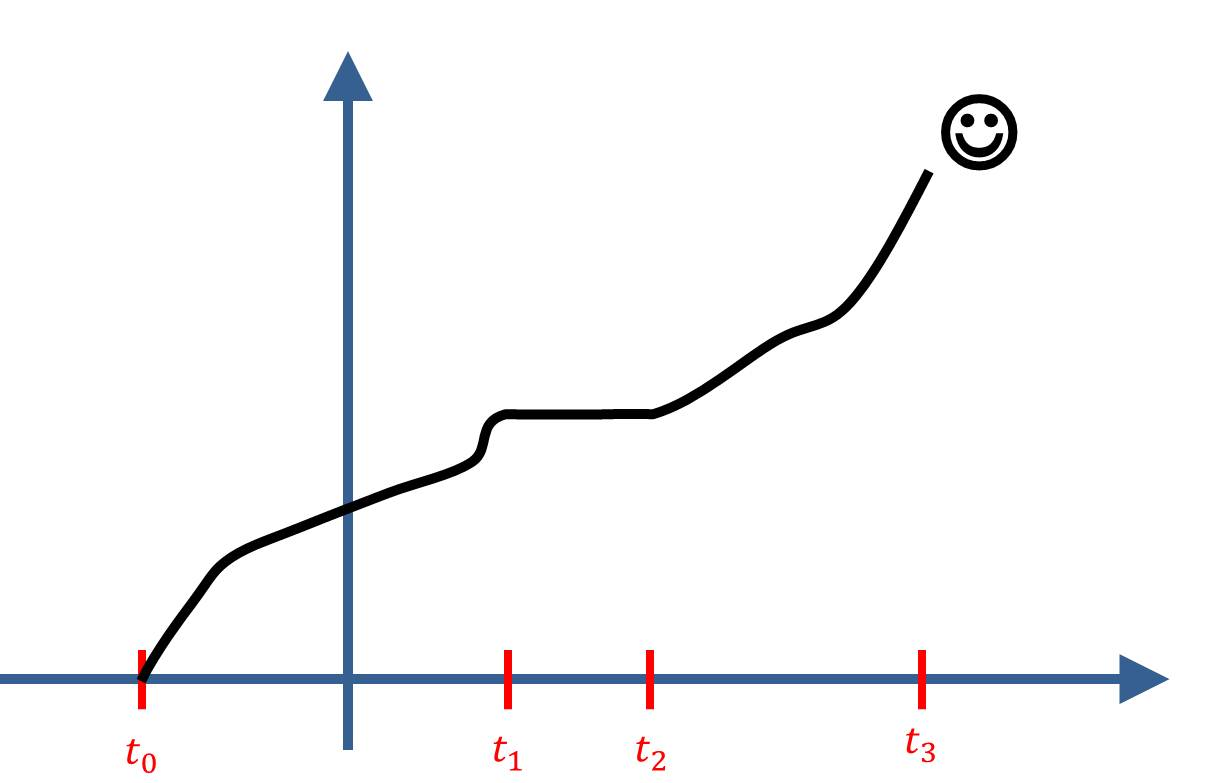
\includegraphics[scale=0.3]{images/Waffel_unzshgd_Fkt.jpg}
\newline
Bei unzusammenhängenden Waffeln ist die Schnittgerade selbst bei vorgegebener Schnittrichtung nicht eindeutig.
\end{example}

\begin{Kasten}{Weg, Anfangspunkt, Endpunkt}
	ein \underline{Weg} in einem topologischen Raum $X$ ist eine stetige Abbildung $\gamma \colon [0,1] \rightarrow X$, und $\gamma(0)$ heißt \underline{Anfangs-}, $\gamma(1)$ \underline{Endpunkt}.
	\newline
\end{Kasten}
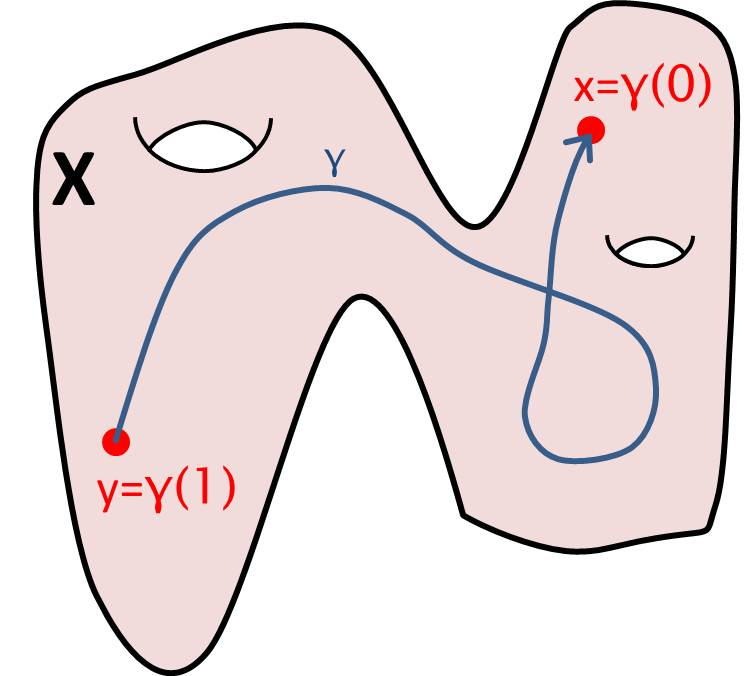
\includegraphics[scale=0.4]{images/Weg.jpg}

\begin{Kasten}{Wegzusammenhang}
	$X$ heißt \underline{wegzusammenhängend} $:\Leftrightarrow$ Zu je zwei Punkten $x,x^\prime \in X \exists \text{ Weg } \gamma \colon [0,1] \rightarrow X \text{ mit } \gamma(0)=x, \gamma(1)=x^\prime$.
	\newline
\end{Kasten}
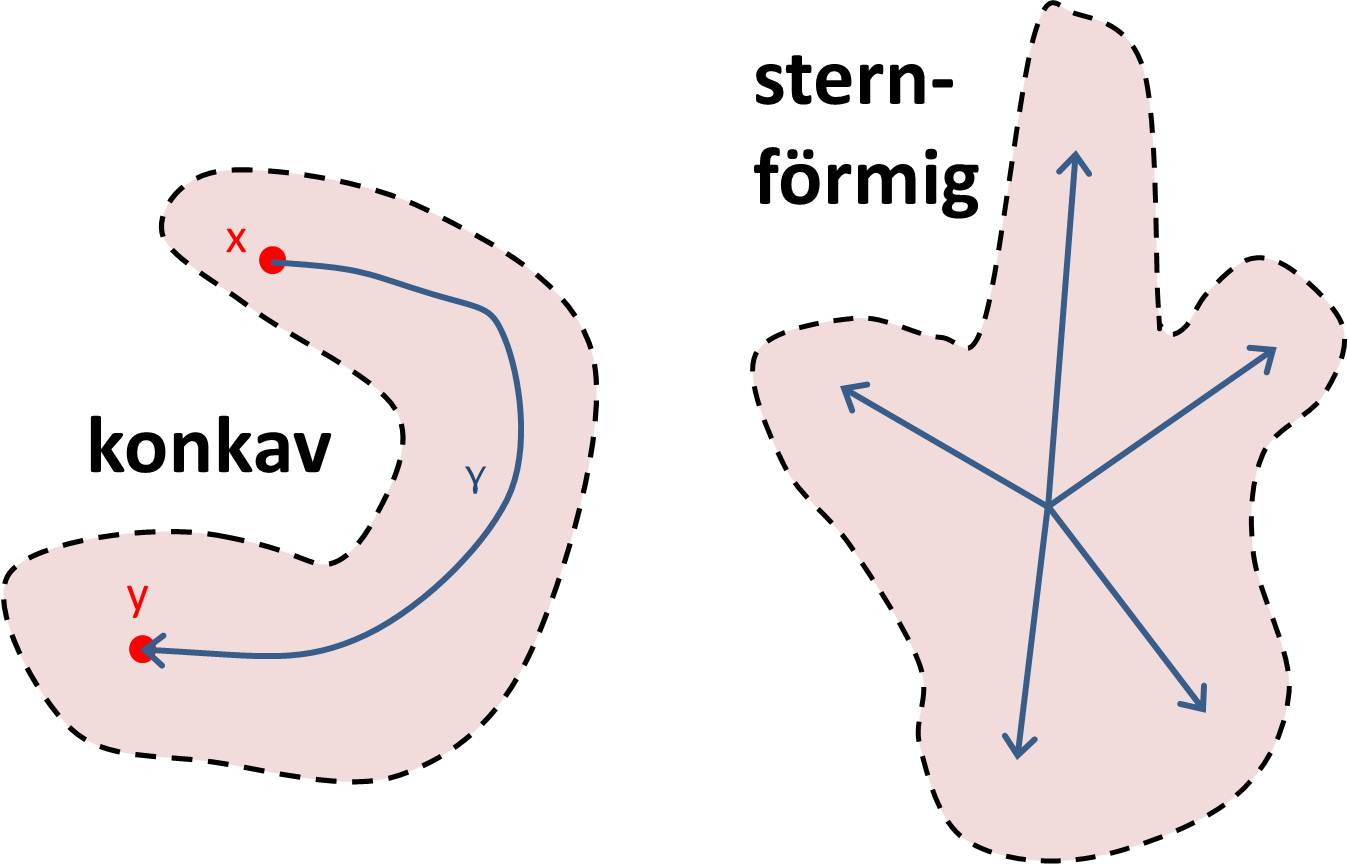
\includegraphics[scale=0.4]{images/Wegzshgd.jpg}

\begin{example}
	$$A=\{(x,y) \in \R^2 \mid x>0, y = \sin{\frac{1}{x}}\} \subset \R^2$$
	$$B=A \cup \{(0,0)\}$$
	$\Rightarrow B$ ist zusammenhängend, aber \underline{nicht} wegzusammenhängend.
	\newline
	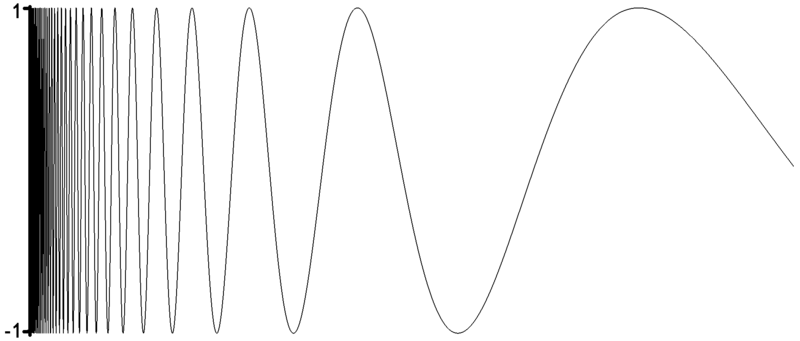
\includegraphics[scale=0.4]{images/Sinuseinsdurchx.png}
	\newline
	\scriptsize{Bild: http://de.wikipedia.org/w/index.php?title=Datei:Sinuseinsdurchx.png\&filetimestamp=20080624085708}
\end{example}

\begin{Kasten}{Kompaktheit}
	Ein topologischer Raum $X$ heißt \underline{kompakt}, falls jede offene Überdeckung von $X$ eine endliche Teilüberdeckung enthält.
\end{Kasten}

\section{Trennungseigenschaften}
\begin{Kasten}{$T_1$-Raum}
Ein topologischer Raum $X$ heißt \underline{$T_1$-Raum} bzw. \underline{erfüllt das erste Trennungsaxiom} $:\Leftrightarrow$ Für je zwei verschiedene Punkte von $X$ existiert für jeden dieser Punkte eine Umgebung in $X$, die den anderen nicht enthält.
\newline
$\forall x \neq y \in X \exists U = U_X \colon y \notin U_X$ 
\end{Kasten}
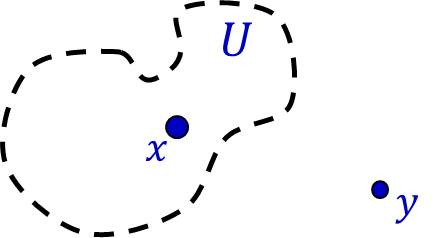
\includegraphics[scale=0.4]{images/T1.jpg}

\begin{Kasten}{$T_2$-Raum}
	$X$ heißt \underline{Hausdorff}- oder \underline{$T_2$-Raum} bzw. \underline{erfüllt das zweite Trennungsaxiom} $:\Leftrightarrow$ Je zwei verschiedene Punkte in $X$ besitzen disjunkte Umgebungen.
	\newline
	$\forall x \neq y \in X \exists U_x \ni x, U_y \ni y$ mit $U_x \cap U_y = \emptyset$
\end{Kasten}
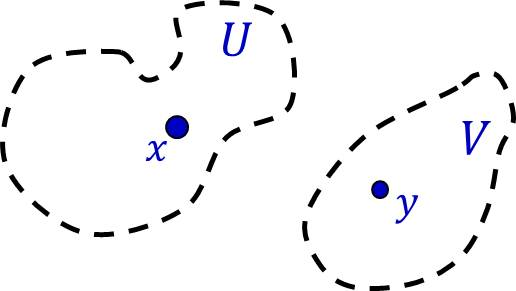
\includegraphics[scale=0.4]{images/T2.jpg}

\begin{example}
	Jeder metrische Raum ist Hausdorff-Raum.
\end{example}

\begin{remark}
Hausdorff-Räume sind z.B. deshalb wichtig, weil Grenzwerte dort eindeutig sind!
\end{remark}

\begin{Kasten}{Grenzwert}
Ist $(x_n)_{n \in \N}$ eine Folge von Punkten in einem topologischen Raum $X$, so heißt $x \in X$ \underline{Grenzwert} der Folge $(x_n)$ genau dann, wenn zu jeder Umgebung $U$ von $x$ ein $N \in \N$ existiert mit $x_n \in U \forall n \geq N$. 
\newline
\end{Kasten}
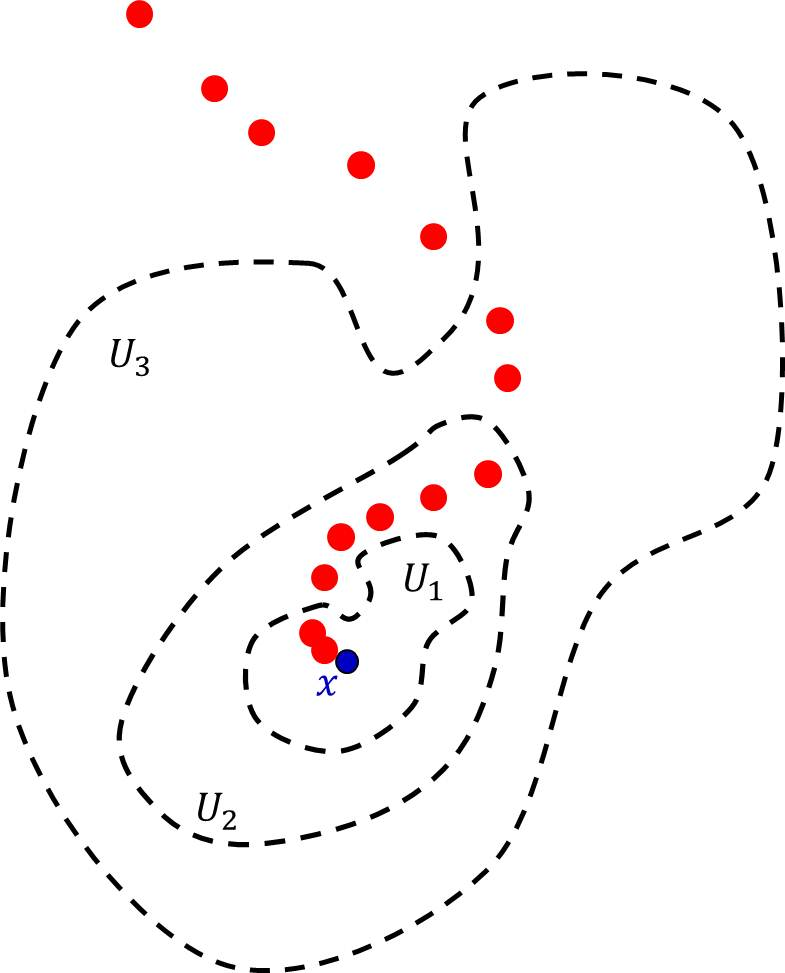
\includegraphics[scale=0.5]{images/Grenzwert.jpg}

\begin{example}
In einem Hausdorff-Raum hat jede Folge höchstens einen Grenzwert.
\end{example}

\begin{remark}
Hausdorff-Räume sind auch $T_1$-Räume, aber:
\end{remark}

\begin{example}
	In $X=\R_{\mathcal{T}_1}$ ist jeder Punkt abgeschlossen ($\Rightarrow T_1$), doch je zwei nichtleere offene Mengen schneiden sich - $X$ ist damit nicht $T_2$!
	%newline
	\underline{"Schlimmer":} In $\R_{\mathcal{T}_1}$ ist \underline{jeder} Punkt Grenzwert der Folge $x_n = n$!
	Denn eine Umgebung eines Punktes in $\R_{\mathcal{T}_1}$ hat die Form $U = \R \backslash \{x_1, \ldots, x_M\}$ mit $x_1 < \ldots < x_M$. Dann gilt aber $x_n = n \in U \forall n > x_M$.
\end{example}

\section{Abzählbarkeitsaxiome}
\begin{Kasten}{Umgebungsbasis}
	Ist $X$ topologischer Raum und $x \in X$, so ist eine \underline{Umgebungsbasis} oder \underline{Basis von $X$} \underline{\underline{in $x$}} eine Familie von Umgebungen von $x$, sodass \underline{jede} Umgebung von $x$ eine Umgebung aus der Familie enthält.
\end{Kasten}

\begin{example}
	Ist $B$ Basis der Topologie eines Raumes $X$, so ist für jedes $x \in X$ $\{U \in B \mid x \in U\}$ eine Basis von $X$ \underline{\underline{in $x$}}.
\end{example}

\begin{example}
	In einem \underline{metrischen} Raum $X$ sind folgende Mengen von Bällen Basen von $X$ in $x \in X$:
	\begin{itemize}
		\item alle offenen Bälle mit Zentrum $x$
		\item alle offenen Bälle mit Zentrum $x$ und rationalen Radii
	\end{itemize}
\end{example}

\begin{example}
	\label{UmgebungsbasisDiskreteTopologie}
	Ist $X$ mit der diskreten bzw. trivialen Topologie versehen, so ist die `kleinste' Basis in $x \in X$ gegeben durch $\left\{\{x\}\right\}$ bzw. $\{X\}$.
\end{example}

\begin{Kasten}{Abzählbarkeitsaxiome, Separabilität}
	$X$ \underline{erfüllt das erste Abzählbarkeitsaxiom}
	$:\Leftrightarrow$ jeder Punkt $x \in X$ besitzt eine abzählbare Basis.
	\newline
	$X$ \underline{erfüllt das zweite Abzählbarkeitsaxiom}
	$:\Leftrightarrow$ $X$ selbst besitzt eine abzählbare Basis.
	\newline
	$X$ heißt \underline{separabel} $:\Leftrightarrow$ $X$ enthält eine abzählbare und dichte ($\bar{A} = X$) Menge $A$.
\end{Kasten}
 
\begin{remark}
	Das zweite Abzählbarkeitsaxiom impliziert das erste, aber:
\end{remark} 

\begin{example}
	Überabzählbare diskrete Räume (wie $(\R, \OO_{diskret})$) erfüllen nach Beispiel~\ref{UmgebungsbasisDiskreteTopologie} das erste Abzählbarkeitsaxiom, nicht aber das zweite!
\end{example}
 
\begin{remark}
	Jeder metrische Raum erfüllt das erste Abzählbarkeitsaxiom und jeder \underline{separable} metrische Raum auch das zweite.
\end{remark} 
 
\begin{example}
	$\R_{\mathcal{T}_1}$ erfüllt \underline{nicht} das erste Abzählbarkeitsaxiom, ist aber separabel - $\N$ ist dicht!
\end{example} 
 
\begin{example}
	Euklidische Räume und alle ihre Teilmengen erfüllen das 2. Abzählbarkeitsaxiom und sind separabel.
\end{example} 
 
Wozu das Ganze? 
\newline $\rightsquigarrow$ Funktionenräume
\newline $\rightsquigarrow$ Mannigfaltigkeiten
\newline $\rightsquigarrow$ \underline{Satz von Lindelöf:}
Jede offene Überdeckung eines Raumes, der das zweite Abzählbarkeitsaxiom erfüllt, enthält auch eine abzählbare \underline{Teilüberdeckung}.
 
\begin{Kasten}{Lokale Kompaktheit}
$X$ heißt \underline{\underline{lokal} kompakt} \newline $:\Leftrightarrow$ Jeder Punkt $x \in X$ besitzt eine Umgebung $U$, sodass $\overline{U}$ kompakt ist.
\end{Kasten} 

\begin{Kasten}{Lokale Endlichkeit}
	Eine Familie $\Gamma$ von Teilmengen eines topologischen Raumes $X$ heißt \underline{lokal endlich} $:\Leftrightarrow \forall x \in X \exists U = U(x) \colon A \cap U = \emptyset \forall A \in \Gamma$ bis auf endlich viele $A$.
\end{Kasten}
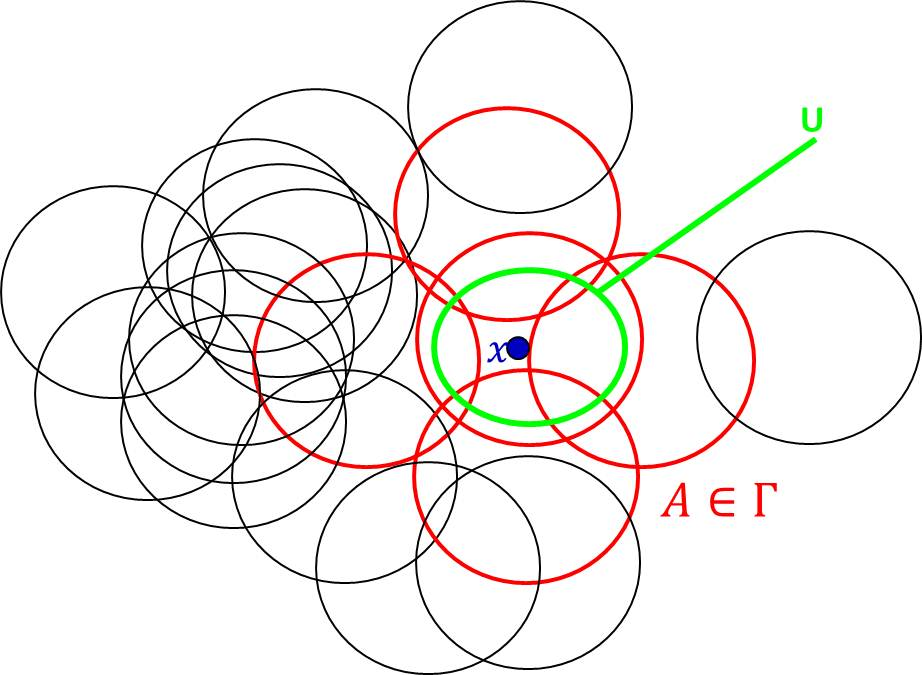
\includegraphics[scale=0.5]{images/lokal_endlich.jpg}
 
\begin{Kasten}{Verfeinerung}
	$\Gamma, \Delta$ Überdeckungen von $X$. $\Delta$ heißt \underline{Verfeinerung} von $\Gamma$ \newline $:\Leftrightarrow \forall A \in \Delta \exists B \in \Gamma \colon A \subset B$.
\end{Kasten} 

\begin{Kasten}{Parakompaktheit}
	$X$ heißt \underline{parakompakt} $:\Leftrightarrow$ Jede offene Überdeckung besitzt eine lokal endliche offene Verfeinerung. 
\end{Kasten}


\includegraphics[scale=0.5]{images/Cutoff.jpg} \underline{\underline{Cut-off}}

%hier beginnt der 10.11.11
\chapter{Beispiele und Konstruktionen topologischer Räume}
\section{Mannigfaltigkeiten}

\paragraph{Beispiele zu Mannigfaltigkeiten (Exkurs)} Doppelpendel, Quantenfeldtheorie

\includegraphics[scale=0.3]{images/Mannigfaltigkeiten1.jpg} \newline \newline
\includegraphics[scale=0.4]{images/S1_Pendel.jpg} \newline \newline
\includegraphics[scale=0.4]{images/Torus_Doppelpendel.jpg} \newline \newline
\includegraphics[scale=0.4]{images/Stringtheorie.jpg}

\begin{Kasten}{Mannigfaltigkeit, Karte}
	Ein topologischer Raum $M$ heißt \underline{$n$-dimensionale} \underline{(topologische) Mannigfaltigkeit}, wenn gilt:
	\begin{enumerate}
		\item $M$ ist ein Hausdorff-Raum mit abzählbarer Basis der Topologie
		\item $M$ ist lokal homöomorph zu $\R^n$, d.h. zu jedem $p \in M$ existieren eine Umgebung $U=U(p) \subset_{offen} M$ und ein Homöomorphismus $\varphi \colon U \rightarrow V, V \subset_{offen} \R^n$.
			\newline
			Jedes solche Paar $(U,\varphi)$ heißt eine \underline{Karte} oder ein \underline{lokales Koordinatensystem} um $p$.
	\end{enumerate}
\end{Kasten}
\includegraphics[scale=0.4]{images/Karte.jpg} 
 
\begin{remark}
	Die Zahl $n$, die \underline{Dimension von $M$}, ist eindeutig bestimmt!
	(folgt aus Brouwers Satz von der Invarianz des Gebietes) 
\end{remark}

\begin{Kasten}{Atlas}
	Ein \underline{Atlas} für eine topologische $n$-Mannigfaltigkeit $M$ ist eine Menge $\mathcal{A} = \{(\varphi_\alpha, U_\alpha) \mid \alpha \in \Lambda\}$\footnote{$\Lambda$ Indexmenge}
	von Karten $\varphi_\alpha \colon U_\alpha \rightarrow V_\alpha = \varphi(U_\alpha) \subset \R^n$, so dass $M = \bigcup\limits_{a \in \Lambda}{U_\alpha}$
\end{Kasten}

\begin{Kasten}{$C^k$-Atlas, Kartenwechsel}
	Ein Atlas heißt \underline{differenzierbar} \underline{von der Klasse $C^k$} (oder: $C^k$-Atlas von $M$), wenn für alle $\alpha, \beta \in \Lambda$ mit $U_\alpha \cap U_\beta \neq \emptyset$ der \underline{Kartenwechsel} $\varphi_\beta \circ \varphi_\alpha^{-1} \colon \varphi_\alpha(U_\alpha \cap U_\beta) \rightarrow \varphi_\beta(U_\alpha \cap U_\beta)$ eine $C^k$-Abbildung, also $k$-mal stetig differenzierbar ist. $(k=0,1,2,\ldots,\infty,\omega)$
	\newline
\end{Kasten}
\includegraphics[scale=0.4]{images/Kartenwechsel.jpg}
 
\begin{Kasten}{Verträglichkeit, differenzierbare Struktur}
	Ist $M$ topologische Mannigfaltigkeit und $\mathcal{A}=\{(\varphi_\alpha,U_\alpha) \mid \alpha \in \Lambda\}$ ein $C^k$-Atlas von $M$, so heißt eine Karte $(\varphi,U)$ von $M$ \underline{mit $\mathcal{A}$ verträglich}, falls $\mathcal{A}^\prime := \mathcal{A} \cup \{(\varphi,U)\}$ ebenfalls $C^k$-Atlas ist. 
	Ein $C^k$-Atlas heißt \underline{maximal} (oder \underline{differenzierbare Struktur} (der Klasse $C^k$)), falls $\mathcal{A}$ alle mit $\mathcal{A}$ verträglichen Karten enthält.
\end{Kasten} 

\begin{Kasten}{$C^k$-Mannigfaltigkeit, glatt}
	Eine \underline{differenzierbare Mannigfaltigkeit der Klasse $C^k$} (kurz: $C^k$-Mannigfaltigkeit) ist ein Paar $(M,\mathcal{A})$ bestehend aus einer topologischen Mannigfaltigkeit $M$ und einer $C^k$-Struktur auf $M$. Eine $C^\infty$-Mannigfaltigkeit heißt auch \underline{\underline{glatt}}.
	\newline
\end{Kasten}
\includegraphics[scale=0.4]{images/Verkleben.jpg}
\includegraphics[scale=0.4]{images/Verkleben_S2.jpg}
\includegraphics[scale=0.4]{images/Norm_invers.jpg}


\paragraph{Richtig toller Exkurs zu Mannigfaltigkeiten}... Killing-Fields, Lie-Groups (festgenommener Matheprof kurz nach 9/11), Perverse Garben, wir leben in einer 4-dimensionalen Mannigfaltigkeit, ...

\newpage
\section{Produkt-Topologie}
\begin{Kasten}{Produkt-Topologie}
	Sind $(X, \OO_X)$ und $(Y, \OO_Y)$ topologische Räume, so bildet $$\mathcal{B}_{X \times Y} := \{U \times V \mid U \in \OO_X, V \in \OO_Y\}$$
	die Basis einer Topologie für die Menge $X \times Y$, und diese heißt \underline{Produkt-Topologie auf $X \times Y$}.
	\newline
	Versehen mit der Produkt-Topologie ist $X \times Y$ sebst ein topologischer Raum und für gegebene $X, Y$ denkt man sich $X \times Y$ stillschweigend mit der Produkt-Topologie versehen.
\end{Kasten}

\begin{example}
	$\R \times \R = \R^2$ \includegraphics[scale=0.06]{images/offener_Kreis.jpg}
	als topologische Räume!
\includegraphics[scale=0.4]{images/Produkt_RxR.jpg} 
\includegraphics[scale=0.4]{images/Kreis_Rechteck.jpg} 
\includegraphics[scale=0.4]{images/Kreis_Rechteck_Basis.jpg} 
	Ebenso: $(\R^1)^n = \R^n$!
\end{example}

\paragraph{Einige Eigenschaften der Produkt-Topologie}
\begin{itemize}
	\item Produkte von Hausdorff-Räumen sind Hausdorff-Räume.
	\item Produkte von zusammenhängenden Räumen sind zusammenhängend.
	\item Produkte von wegzusammenhängenden Räumen sind wegzusammenhängend.
	\item Produkte von kompakten/separablen Räumen sind kompakt/separabel.
	\item Produkte von Räumen, die das erste oder zweite Abzählbarkeitsaxiom erfüllen, erfüllen diese auch.
\end{itemize}
 
\begin{example}
	Produkte topologischer oder differenzierbarer Mannigfaltigkeiten sind topologische oder differenzierbare\footnote{($C^\infty$)} Mannigfaltigkeiten.
\end{example} 
 
\begin{example}
	\begin{itemize}
		\item $\R^2 \backslash \{0\} \cong S^1 \times \R^{> 0}$ (Polarkoordinaten) \newline
		\includegraphics[scale=0.4]{images/Polarkoordinaten.jpg}
		\item $O(n) \cong SO(n) \times O(1)$
		\item $(S^1)^n :=  \underbrace{S^1 \times \ldots \times S^1}_{\text{n mal}}$ heißt \underline{n-dimensionaler Torus} (TODO: Bild 3: Exkurs höherdimensionale Sphären)
	\end{itemize}
\end{example}

\section{Differenzierbare Abbildungen}
\begin{Kasten}{$C^l$-Abbildung}
Es seien $(M, \mathcal{A})$ eine $n$-dimensionale $C^k$-Mannigfaltigkeit, $(M^\prime, \mathcal{A}^\prime)$ eine $n^\prime$-dimensionale $C^{k^\prime}$-Mannigfaltigkeit und $l \leq \min(k,k^\prime)$. Eine stetige Abbildung $f \colon M \rightarrow M^\prime$ heißt \underline{differenzierbar} (\underline{von der Klasse $C^l$}) oder kurz: $C^l$-Abbildung, falls gilt:
$$\forall (\varphi,U) \in \mathcal{A} \text{ und } (\varphi^\prime, U^\prime) \in \mathcal{A}^\prime \text{ mit } f(U) \cap U^\prime \neq \emptyset \text{ ist}$$
$$\boxed{\varphi^\prime \circ f \circ \varphi^{-1} \colon \varphi(U \cap f^{-1}(U^\prime)) \rightarrow \varphi^\prime(f(U)\cap U^\prime)}$$
eine $C^l$-Abbildung im üblichen Sinn.
\end{Kasten}
\includegraphics[scale=0.5]{images/Abb_diffbar.jpg}
 
TODO: Exkurs über Tangentialvektoren, Vektorfelder, Satz vom Igel, Physik des starren Körpers, Differentialtopologie

\paragraph{
Spezielle Mannigfaltigkeiten: Untermannigfaltigkeiten topologischer Räume: }
 
\begin{theorem}[Äquivalente Beschreibungen einer Untermannigfaltigkeit von $\R^{n+l}$]
	Für Teilmengen $M \subset \R^{n+l}$ sind äquivalent:
	\begin{enumerate}[(a)]
		\item $\forall x_0 \in M \exists \text{ Umgebung } U = U(x_0) \subset_{offen} \R^{n+l}$ und $$f \in C^\infty(U, \R^l) := \{g \colon U \rightarrow \R^l \mid g \text{ ist } C^\infty\}\text{ mit Rang }Df(x) = l \quad \forall x \in U$$ \footnote{$Df$ ist die Jacobi-Matrix von $f$} dergestalt, dass $U \cap M = f^{-1}(0) = \{x \in U \mid f(x) = 0\}$ 
\includegraphics[scale=0.5]{images/Satz_UnterMf.jpg}
		\item $\forall x_0 \in M \exists U = U(x) \subset_{offen} \R^{n+l}$ und $\varphi \colon U \rightarrow \R^{n+l}$ mit folgenden Eigenschaften:
		$\varphi(U) \subset \R^{n+l}$ ist offen, $\varphi$ ist $C^\infty$-Diffeomorphismus $U \rightarrow \varphi(U)$ und $$\varphi(U \cap M) = \varphi(U) \cap (\R^n \times \{0\}) = \{(y_1, \ldots, y_{n+l}) \in \varphi(U) \mid y_{n+1} = \ldots = y_{n+l} = 0 \}$$
		\item $\forall x_0 \in M \exists U = U(x_0) \subset_{offen} \R^{n+l}, W \subset \R^n$ offen und $\psi \in C^\infty(W,U)$ mit 
			\begin{itemize}
				\item $\psi$ ist Homöomorphismus $W \rightarrow U \cap M$
				\item $D\psi(w)$ ist injektiv für alle $w \in W$
			\end{itemize}
			(Jedes solche $\psi$ heißt \underline{lokale Parametrisierung von $M$}).
	\end{enumerate}
\end{theorem}

\paragraph{Interpretation}
\begin{enumerate}[(a)]
	\item besagt: $U \cap M$ ist (im Sinne der Rangbedingung) durch $l$ unabhängige Gleichungen $f_1(x) = \ldots = f_l(x) = 0$ definiert.
	\item besagt: nach Anwendung eines Diffeomorphismus sieht $U \cap M$ wie eine offene Teilmenge eines linearen Unterraumes von $\R^{n+l}$ aus.
	\item besagt: $M$ lässt sich lokal parametrisieren.
\end{enumerate}

\begin{Kasten}{Untermannigfaltigkeit}
Eine Menge $M \subset \R^{n+l}$, die eine der Bedingungen (a), (b) oder (c) erfüllt, heißt dann \underline{$n$-dimensionale} \underline{(glatte/differenzierbare) Untermannigfaltigkeit von $\R^{n+l}$}.
\end{Kasten}

%hier beginnt der 17.11.

\begin{theorem}{Äquivalente Beschreibung einer glatten Untermannigfaltigkeit von $\R^{n+l}$}
	Es sei $M \subseteq \R^{n+l}$. Es sind äquivalent:
	\begin{enumerate}[(a)]
		\item $\forall x_0 \in M \exists U = U(x_0) \subseteq_{\text{offen}} \R^{n+l} \text{ und } f \in C^\infty(U,\R^l)$ $\text{ mit Rang }Df(x) = l \text{ für alle } x \in U$ dergestalt, dass $U \cap M = f^{-1}(0)$.
		\item $\forall x_0 \in M \exists U = U(x) \subseteq_{\text{offen}} \R^{n+l} \text{ und } \varphi \colon U \rightarrow \R^{n+l}$ mit folgenden Eigenschaften:
			\begin{itemize}
				\item $\varphi(U) \subseteq \R^{n+l}$ ist offen
				\item $\varphi$ ist $C^\infty$-Diffeomorphismus $U \rightarrow \varphi(U)$
				\item $\varphi(U \cap M) = \varphi(U) \cap (\R^n \times \{0\})$ $= \{(y_1, \ldots, y_n) \in \varphi(U) \mid y_{n+1} = \ldots = y_{n+l} = 0\}$
			\end{itemize}
		\item $\forall x_0 \in M \exists U = U(x_0) \subseteq_{\text{offen}} \R^{n+l}$, $W \subseteq \R^n$ offen und $\psi \in C^\infty(W,U)$ mit folgenden Eigenschaften:
			\begin{itemize}
				\item $\psi$ ist Homöomorphismus $W \rightarrow U \cap M$
				\item $D\psi(w)$ ist injektiv für alle $w \in W$.
			\end{itemize}
	\end{enumerate}
\end{theorem}

\begin{example}
	\underline{zu (a)}
	\newline
	Die $n$-Sphäre vom Radius $r$ %TODO: r=0, r<0?
	$$S_r^n = \{x \in \R^{n+1} \mid ||x|| = r\}$$
	ist eine $n$-dimensionale glatte Untermannigfaltigkeit von $\R^{n+1}$.
	\newline
	\underline{Denn:}
	Definiere $f \colon \R^{n+1} \rightarrow \R, x \mapsto ||x||^2 - r^2$.
	Dann gilt:
	\begin{itemize}
		\item $S_r^n = f^{-1}(0)$ und
		\item $Df(x) = (2x_1, \ldots, 2x_{n+1}) = 2x$
	erfüllt Rang $Df(x)=1$ für alle $x \in \R^{n+1}\backslash\{0\} \supseteq S_r^n$ (wegen $||x||=\sqrt{x_1^2+\dotsb+x_{n+1}^2}$).
		\end{itemize}
		
	Allgemeiner:
	\begin{itemize}
		\item \underline{Niveaumengen:}
			Es seien $V \subseteq_{\text{offen}} \R^{n+l}, f \in C^\infty(V, \R^l), c \in \R^l$.
			Gilt Rang $Df(x) = l$ in jedem Punkt $x$ der \underline{Niveaumenge} $$f^{-1}(c)=\{x \in V \mid f(x)=c\},$$ so ist $f^{-1}(c)$ eine glatte $n$-dimensionale Untermannigfaltigkeit von $\R^{n+l}$.
	\end{itemize}
\end{example}

\begin{proof}
		\underline{(a)$\Rightarrow$(b):} Es seien $U$ und $f$ wie in (a) gewählt und $f_1, \ldots, f_l$ die Komponenten von $f$. Sei $x_0 \in M$. Durch Umnummerierung seien die Indizes so gewählt, dass ohne Einschränkung die Reihenfolge so, dass die $(l \times l)$-Matrix 
		$$\left(\frac{\partial f_i}{\partial x_{n+j}}\right)_{i,j \in \{1, \ldots, l\}}$$
		in $x_0$ invertierbar ist.
		Definiere die Abbildung $\varphi \colon U \rightarrow \R^{n+l}, x \mapsto (x_1, \ldots, x_n, f_1(x), \ldots, f_l(x))$.
		Dann gilt:
		$$D \varphi(x_0)= (TODO:Matrix 2)$$ und damit 
		$$\det{D \varphi(x_0)} = \det{\left(\frac{\partial f_i}{\partial x_{n+j}}\right)_{i,j}} \neq 0.$$
		Mit dem Satz über inverse Funktionen (oder "Satz über die Umkehrabbildung") folgt:
		Es existieren Umgebungen $U^\prime = U^\prime(x_0) \subseteq U$ und $V^\prime(\varphi(x_0)) \subseteq V = \varphi(U)$, so dass
		$\varphi \big |_{U^\prime} \colon U^\prime \rightarrow V^\prime$ ist $C^\infty$-Diffeomorphismus.
		\newline
		Es gilt: $\varphi(U^\prime \cap M) = \{(y_1, \ldots, y_{n+l}) \in \varphi(U^\prime) \mid y_{n+1} = \ldots = y_{n+l}=0\}$,
		\underline{denn:} \newline $"\subseteq":$ ist klar nach Definition von $f$ und $\varphi$.
		\newline
		$"\supseteq":$ Ist $y$ Element der rechten Seite, so existiert $x \in U^\prime$ mit $\varphi(x)=y$ und $f(x)=0$. Da $x \in U^\prime \subseteq U$ und $f(x)=0$, gilt: $x \in U^\prime \cap M$, und damit $y = \varphi(x) \in \varphi(U^\prime \cap M)$.
		\newline
		 \underline{(b)$\Rightarrow$(c):} Es seien $U$ und $\varphi$ wie in (b) gewählt und
		 $$\pi \colon \R^{n+l} = \R^n \times \R^l \rightarrow \R^n, (x_1, \ldots, x_{n+l}) \mapsto (x_1, \ldots, x_n),$$
		 die \underline{Projektion} und
		 $$\iota \colon \R^n \rightarrow \R^{n+l}, (x_1, \ldots, x_n) \rightarrow (x_1, \ldots, x_n, 0, \ldots, 0)$$ die \underline{Inklusion}.
		 \newline
		 Setze $W := \pi(\varphi(U \cap M))$ und definiere $\psi \colon W \rightarrow U$ durch $\psi := \varphi^{-1} \circ \iota$.
		 \newline
\includegraphics[scale=0.5]{images/Beweis_Satz_UMF_Diagramm.jpg}
		 \newline
		 Dann ist $W$ offen und $\psi \colon W \rightarrow U \cap M$ ein Homöomorphismus, denn $\iota^\prime \colon W \rightarrow \varphi(U \cap M)$ ist Homöomorphismus und $\varphi^{-1} \colon \varphi(U \cap M) \rightarrow U \cap M$ ist Homöomorphismus.
		 \newline
		 Mit der Kettenregel folgt: Für alle $w \in W$ gilt:
		 $$D \psi(w) = D(\varphi^{-1} \circ \iota^\prime)(w) = \underline{(D \varphi^{-1}) (\iota^\prime(w))} \cdot D\iota^\prime (w)$$ 
		 $$\overset{(D \varphi^{-1})(y) = ((D \varphi)(\varphi^{-1}(y)))^{-1}}{=} ((D \varphi) (\varphi^{-1}(\iota^\prime(w))))^{-1} \circ \iota^\prime$$
		 $$= (D \varphi ( \psi(w))^{-1} \circ \iota^\prime.$$
		 Somit ist $D \psi(w)$ als Komposition einer bijektiven und einer injektiven Abbildung injektiv für alle $w \in W$.
		 \newline
		 \underline{(c)$\Rightarrow$(a):} Es seien $U$, $W$ und $\psi$ wie in (c) gewählt und $\psi(\hat{w})= x_0$ für $\hat{w} \in W$.
		 Da Rang $D \psi(\hat{w}) = n$ folgt nach evtl. Umnummerierung
		 $$\left(\frac{\delta \psi_i}{\delta w_j}(\hat{w})\right)_{i,j \in \{1, \ldots, n\}}$$ ist invertierbar.
		 Definiere $g \colon W \times \R^l \rightarrow \R^{n+l}, (w,y) \mapsto \psi(w) + (0,y)$, d.h. $g(w_1, \ldots,w_n,y_1,\ldots,y_l) = (\psi_1(w), \ldots, \psi_n(w), \psi_{n+1}(w)+y_1, \psi_{n+l}(w)+y_l).$
		 Dann gilt: 
		 $$Dy(\hat{w},0)= (TODO:Matrix 4)$$ ist invertierbar.
		 Mit dem Satz über inverse Funktionen folgt:
		 Es existieren Umgebungen $V = V((\hat{w},0)) \subseteq W \times \R^l$ und $U^\prime = U^\prime(g(\hat{w},0))$, so dass $g \big |_V \colon V \rightarrow U^\prime$ ein $C^\infty$-Diffeomorphismus ist. \newline
		 Verkleinert man gegebenenfalls $V$, so kann man ohne Einschränkung annehmen, dass gilt: $U^\prime \subseteq U$.
		 Da $\{w \in W \mid (w,0) \in V\}$ offen ist in $W$ und $\psi \colon W \rightarrow \psi(W)$ nach Voraussetzung ein Homöomorphismus ist, folgt: $\{\psi(w) \mid (w,0) \in V\}$ ist offen in $\psi(W)$.
		 \newline
		 Nach Definition der Unterraumtopologie existiert $U^{\prime\prime} \subseteq_{\text{offen}} \R^{n+l}$ mit $\{\psi(w)\mid(w,0) \in V\} = U^{\prime\prime} \cap \psi(W)$.
		 \newline
		 Wegen $\psi(w)=g(w,0)$ bedeutet dies:
		 $$(*) U^{\prime\prime} \cap \psi(W) = g(V \cap(W \times \{0\})).$$
		 Setze $\tilde{U} := U^\prime \cap U^{\prime\prime}, \tilde{V} := (g \big |_V)^{-1}(\tilde{U}) = g^{-1}(\tilde{U}) \cap V.$
		 Dann ist $g \big |_{\tilde{V}} \colon \tilde{V} \rightarrow \tilde{U}$ ein $C^\infty$-Diffeomorphismus.
		 \newline
		 \underline{Behauptung:} Es gilt: $\tilde{U} \cap M = g(\tilde{V} \cap (\R^n \times \{0\}))$. 
		 \newline
		 \underline{[Beweis:} folgt mit (*)].
		 \newline
		 Ist $\pi \colon \R^{n+l} \rightarrow \R^l, (x_1, \ldots, x_{n+l}) \mapsto (x_{n+1}, \ldots, x_{n+l})$ die Projektion, so erfüllt $f := \pi \circ (g \big |_{\tilde{V}})^{-1} \colon \tilde{U} \rightarrow \R^l$ die Bedingung in (a).
\end{proof}

\begin{theorem}{($C^\infty$-Untermannigfaltigkeiten von $\R^{n+l}$ sind $C^\infty$-Mannigfaltigkeiten)}
	Es sei $M \subseteq \R^{n+l}$ $n$-dimensionale $C^\infty$-Untermannigfaltigkeit von $\R^{n+l}$ und $\{\psi_\alpha \colon W_\alpha \rightarrow U_\alpha \cap M \mid \alpha \in \Lambda\}$ eine Menge lokaler Parametrisierungen (wie in (c)) mit $M \subseteq \bigcup\limits_{\alpha \in \Lambda}{U_\alpha}$.
	Dann ist $\mathcal{A} = \{(\psi_\alpha^{-1}, U_\alpha \cap M) \mid \alpha \in \Lambda\}$ ein $C^\infty$-Atlas und $M$ eine $C^\infty$-Mannigfaltigkeit.
\end{theorem}

% hier beginnt der 22.11.11

(TODO:Bild)
 
\section{Quotientenräume}
\paragraph{Erinnerung} Jede Partition (TODO:Bild) $S$ einer Menge $X$ bestimmt eine Äquivalenzrelation auf $X$ (und umgekehrt).
\newline
Menge der Äquivalenzklassen (oder auch: Quotient von $X$ nach $S$) ist $X/S$.
Zusätzlich existiert dann die Quotientenabbildung $\pi \colon X \rightarrow X/S, x \mapsto [x]$ 

\begin{remark}
	Ist $X$ ein topologischer Raum und $X/S$ ein Quotientenraum von $X$, so gibt es auf $X/S$ eine natürliche Topologie:
\end{remark}

\begin{Kasten}{Quotienten(raum)topologie}
	Eine Teilmenge $U \subset X/S$ heißt \underline{offen}
	$:\Leftrightarrow \pi^{-1}(U)$ ist offen in $X$
\end{Kasten}
 
\begin{remark}
	Alle im Sinne dieser Definition offenen Teilmengen von $X/S$ definieren dann eine Topologie auf $X/S$ und die Menge $X/S$ zusammen mit dieser Topologie heißt \underline{Qotienten\underline{raum}} von $X$ nach $S$.
\end{remark}

\begin{remark}
	$\pi \colon X \rightarrow X/S$, $X/S$ versehen mit der Quotiententopologie, ist dann eine  \underline{stetige} Abbildung zwischen topologischen Räumen.
\end{remark}

\paragraph{Eigenschaften der Quotiententopologie}
\begin{itemize}
	\item Quotientenräume zusammenhängender Räume sind zusammenhängend.
	\item Quotientenräume wegzusammenhängender Räume sind wegzusammenhängend.
	\item Quotientenräume separabler Räume sind separabel.
	\item Quotientenräume kompakter Räume sind kompakt.
\end{itemize}

\paragraph{Achtung:}
Die Hausdorff-Eigenschaft vererbt sich i.a. nicht!

\begin{example}
	$X = \R, \quad S:= \{\R^{>0}, \R \backslash \R^{>0}\}$
	(TODO: Bild)(TODO:Bild)
	\newline
	$\alpha \in \R \backslash \Q$: \underline{\underline{ÜBEL!}}
	(TODO:Bild)
	\newline
	$t \mapsto e^{2 \pi i t}$
	\newline
	$T^2$ ist Hausdorffsch, $T^2/\textcolor{red}{\sim \underline{nicht}!}$
\end{example}

\paragraph{TODO: Exkurs: Instabilität von Planetensystemen}



\section{Quotientenabbildungen}
Ist $S$ eine Partition von $X$ in nichtleere disjunkte Teilmengen und $f \colon X \rightarrow Y$ eine Abbildung, die auf jedem Element von $S$ konstant ist, so existiert eine Abbildung $X/S \rightarrow Y$, die jedes Element $A$ von $S$ auf $f(a), a \in A,$ abbildet. \newline
\includegraphics[scale=0.4]{images/Quotientenabbildung.jpg} \newline
Diese heißt dann \textbf{Quotientenabbildung} von $f$ nach $S$, in Zeichen $f/S$.

\paragraph{Interpretation}
\includegraphics[scale=0.4]{images/f_modulo_S_Diagramm.jpg}

\paragraph{Allgemeiner}
$S$ Partition von $X$, $T$ Partition von $Y$
\newline
$\Rightarrow$ Jede Abbildung $f \colon X \rightarrow Y$, die jedes Element von $S$ auf ein Element von $T$ abbildet, induziert eine Abbildung 
$$f/_{S,T} \colon X/S \rightarrow Y/T$$
\includegraphics[scale=0.4]{images/f_modulo_S_T_Diagramm.jpg}

\begin{remark}
	Sind $X,Y$ topologische Räume, $S$ Partition von $X$ und $f \colon X \rightarrow Y$ eine auf Elementen von $S$ konstante, \underline{stetige} Abbildung, so ist auch $f/S \colon X/S \rightarrow Y$ stetig.
	\newline
	$f \mapsto f/S$ ist \underline{dann} Bijektion! 
\end{remark}

\paragraph{Erinnerung}
$F \colon X \rightarrow Y$ stetige Bijektion von einem kompakten Raum $X$ auf einen Hausdorff-Raum $Y$ $\Rightarrow$ $F$ ist Homöomorphismus!

\begin{corollary}
	$X$ kompakt, $Y$ Hausdorffsch und $f \colon X \rightarrow Y$ sei stetig 
	$\Rightarrow$ Der \underline{injektive Quotient} $f/_{S(f)}$ ist Homöomorphismus $X/_{S(f)} \rightarrow f(X)$
\end{corollary}

%\paragraph{Beispiel/Definition}
\begin{Kasten}{injektiver Quotient}
\underline{\underline{Jede}} Abbildung $f \colon X \rightarrow Y$ definiert eine Partition $S = S(f)$ von $X$, und zwar in die nichtleeren Urbilder der Elemente von $Y$ unter $f$.
\newline
Die induzierte Abbildung $f/_{S(f)} \colon X/_{S(f)} \rightarrow Y$ ist dann \underline{injektiv} und heißt \underline{injektiver Quotient} von $f$.
\end{Kasten}

\begin{example}
	(TODO: Bild)
	\newline
	$(x,0) \sim (x,1)$
	\newline
	$(0,y) \sim (1,y)$
	\newline
	(TODO: Bild)
	$(x,0) \sim (1-x,1)$
	\newline Möbiusband (TODO: Bild)
\end{example}

\end{document}
